\documentclass[11pt,a4paper]{article}

\usepackage[margin=2.2cm]{geometry}
\usepackage[T1]{fontenc}
\usepackage{lmodern}
\usepackage{graphicx}
\usepackage{booktabs}
\usepackage{amsmath}
\usepackage{float}
\usepackage{caption}
\usepackage{subcaption}
\usepackage{xcolor}
\usepackage{enumitem}
\usepackage[hidelinks]{hyperref}

\graphicspath{{figures/}}
\setlist{itemsep=2pt,topsep=4pt}

% Things the team still has to fill in or check before submitting.
\newcommand{\todo}[1]{\textcolor{red}{\textbf{[TODO: #1]}}}

\title{\textbf{From Pixels to Language}\\[4pt]
\large CSE 485 / CSE 488 Deep Learning --- Final Project Report\\
Milestone 1: Data Understanding and Image Classification}
\author{Mohamed Wael ElHadary \and Kerolos Bassem \and Andrea\\[4pt]
\small Team \todo{team number} \quad
\small Ain Shams University, Faculty of Engineering}
\date{\today}

\begin{document}
\maketitle

\begin{abstract}
We build the first stage of an end-to-end multimodal system on CUB-200-2011
with natural-language captions: a visual encoder trained for 200-way bird
species classification, which later becomes the backbone for colorization and
captioning. We analyse and clean the data, design an augmentation pipeline,
train a CNN from scratch as a baseline, and compare it with ImageNet-pretrained
ResNet-18 encoders used frozen and fine-tuned. The scratch CNN is tuned with
grid search, random search and a coarse-to-fine follow-up. On the official test
split the tuned scratch CNN reaches 49.6\% top-1 accuracy, the frozen ResNet-18
64.3\%, and the fine-tuned ResNet-18 74.4\% (92.3\% top-5). Grad-CAM shows that
the scratch model still relies partly on background cues, while the fine-tuned
model attends to the bird and fails mainly on visually near-identical species.
\end{abstract}

\tableofcontents
\newpage

%=====================================================================
\section{Introduction}
%=====================================================================

The project builds one visual encoder and reuses it for three tasks:
(1) image classification, (2) colorization of grayscale images and
(3) caption generation. This report covers Milestone~1: understanding and
preparing the data, and training the classification encoder.

\paragraph{Dataset choice.} We use the default dataset, CUB-200-2011~\cite{wah2011}
with the captions of Reed et al.~\cite{reed2016}, loaded from Hugging Face
(\texttt{Multimodal-Fatima/CUB\_train} and \texttt{CUB\_test}). It fits all
three tasks: every image has a species label (classification), the photos are
of good quality and can be turned into grayscale/colour pairs (colorization),
and every image has ten human-written descriptions (captioning). At about
1.1\,GB it also fits the free Kaggle T4 GPU we trained on.

\paragraph{Why it is hard.} CUB is a \emph{fine-grained} benchmark: 200 species,
many of which differ only in small details (a wing bar, the colour of a
crown), with only about 30 training images per species. This makes it a good
test of how much a model can learn from little data, and of the value of
transfer learning.

\paragraph{Code.} All final code is pure Python under \texttt{src/} and is run
through one command-line interface (\texttt{python -m src.cli}) with the
sub-commands \texttt{train}, \texttt{evaluate}, \texttt{predict},
\texttt{tune}, \texttt{explain} and \texttt{compare}. Data, models, training,
evaluation and visualization live in separate modules; models are created by a
registry (\texttt{src/models/factory.py}), so the trainer never names a
specific architecture. The exact commands are in the \texttt{README.md}.

%=====================================================================
\section{Data: Analysis, Cleaning and Preprocessing}
%=====================================================================

\subsection{Overview}

\begin{table}[H]
\centering
\caption{Dataset overview (computed by \texttt{src/visualization/eda\_plots.py} and \texttt{eda\_extra.py}).}
\label{tab:data}
\begin{tabular}{lrr}
\toprule
 & Train & Test \\
\midrule
Images & 5,994 & 5,794 \\
Classes & 200 & 200 \\
Images per class (min / mean / max) & 29 / 29.97 / 30 & 11 / 28.97 / 30 \\
Grayscale images (mode \texttt{L}) & 4 & 4 \\
Corrupted / unreadable images & 0 & 0 \\
Median image size (W $\times$ H) & 500 $\times$ 375 & 500 $\times$ 375 \\
Captions per image & 10 (all) & 10 (all) \\
Caption length in words (mean / median / max) & 15.2 / 14 / 65 & 15.2 / 14 / 62 \\
\bottomrule
\end{tabular}
\end{table}

\begin{figure}[H]
\centering
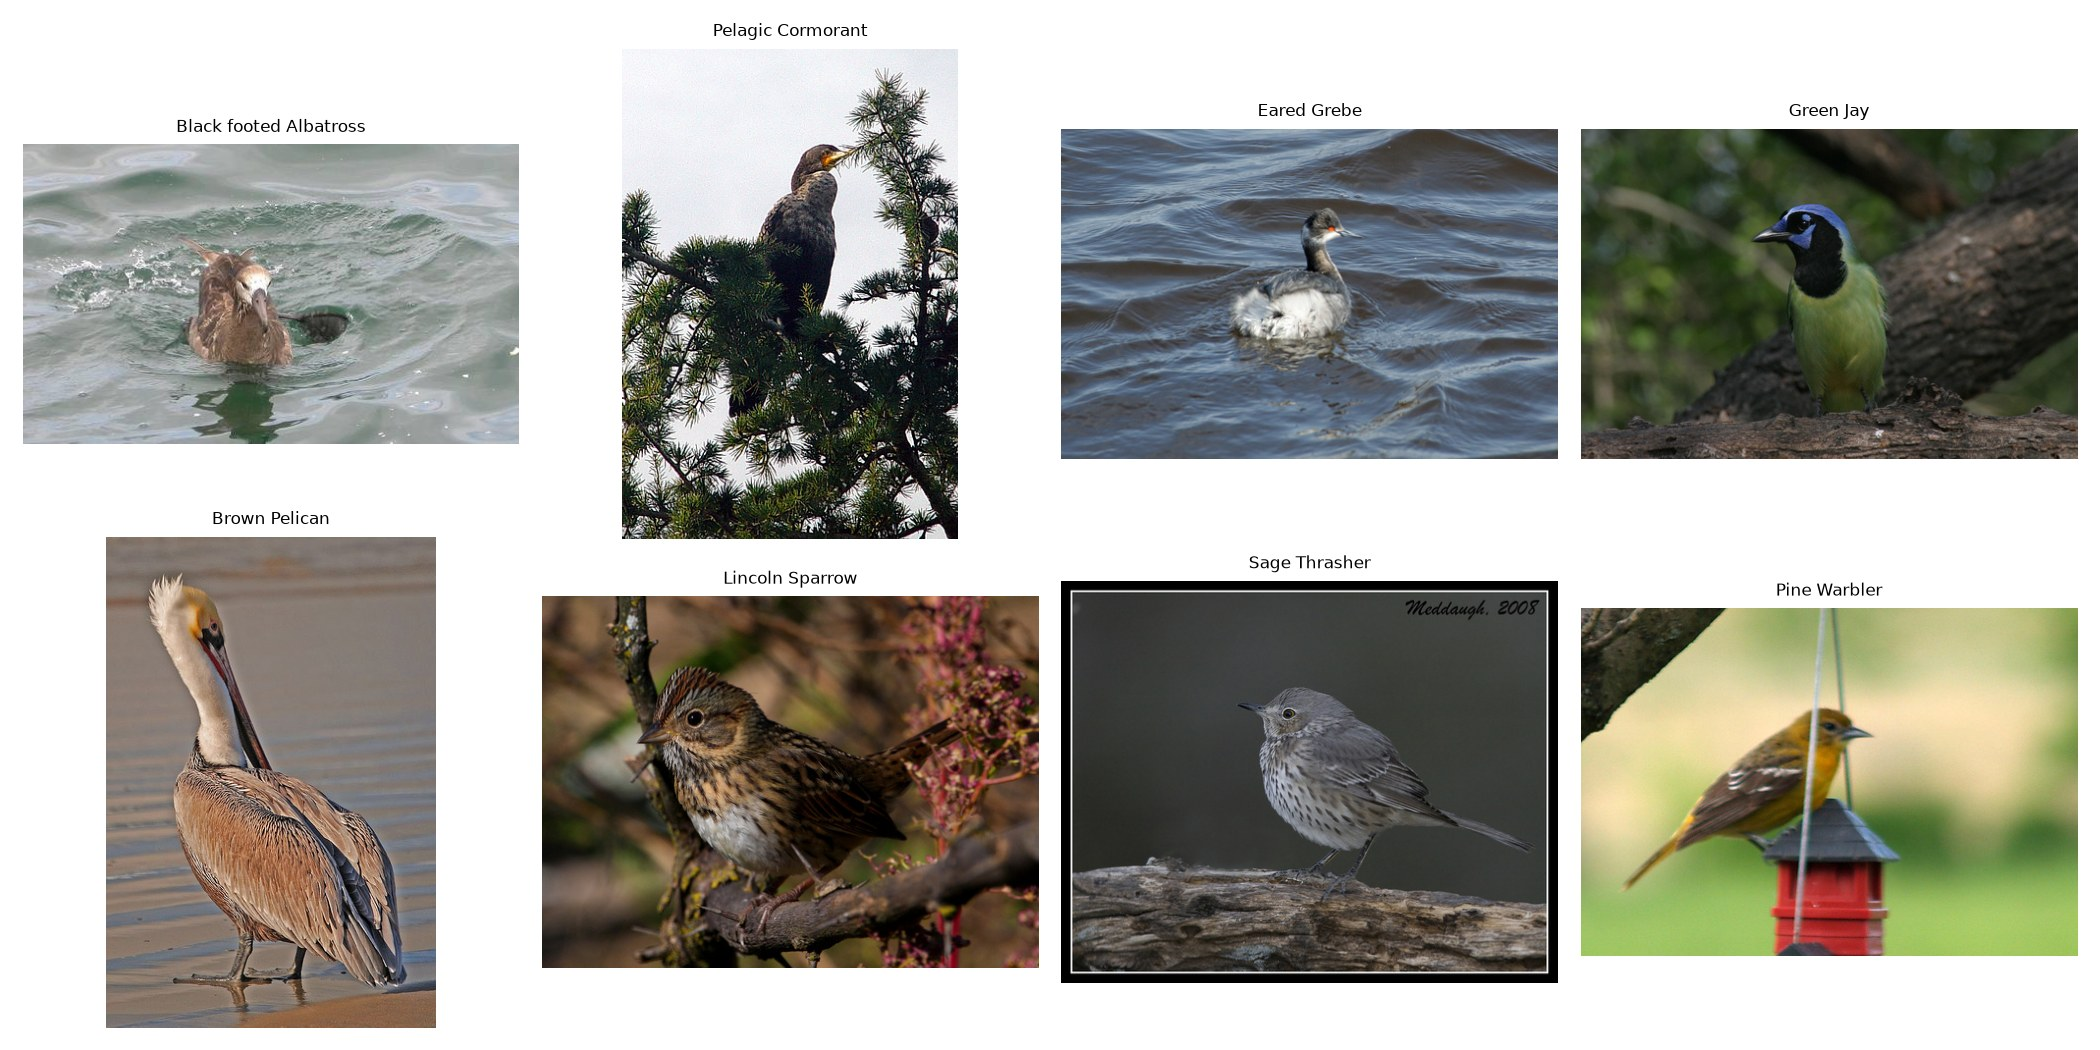
\includegraphics[width=0.95\linewidth]{samples_train.jpg}
\caption{Training samples with their species labels.}
\label{fig:samples}
\end{figure}

\subsection{Class distribution}

The training split is almost perfectly balanced: 194 species have 30 images and
6 have 29 (Figure~\ref{fig:classdist}). The test split is less even (11 to 30
images per class, 52 classes below 30), but no class is missing. Because the
training classes are balanced we use plain cross-entropy without class
weights, and we report \emph{macro}-averaged precision, recall and F1 so that
every species counts equally in the evaluation.

\begin{figure}[H]
\centering
\begin{subfigure}{0.49\linewidth}
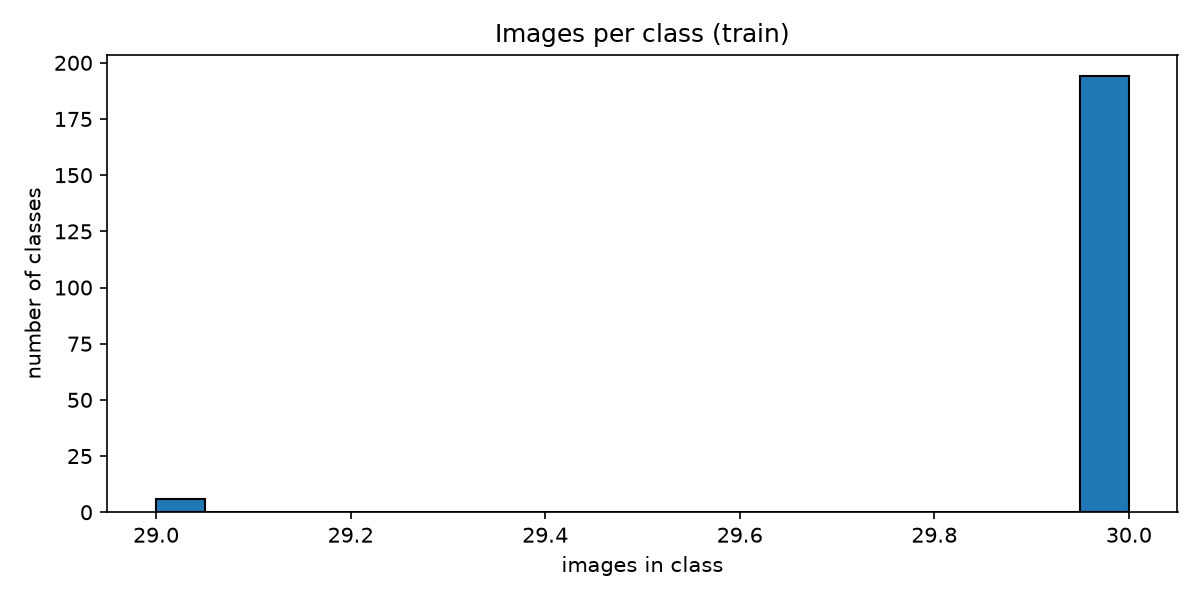
\includegraphics[width=\linewidth]{class_dist_train.png}
\end{subfigure}
\begin{subfigure}{0.49\linewidth}
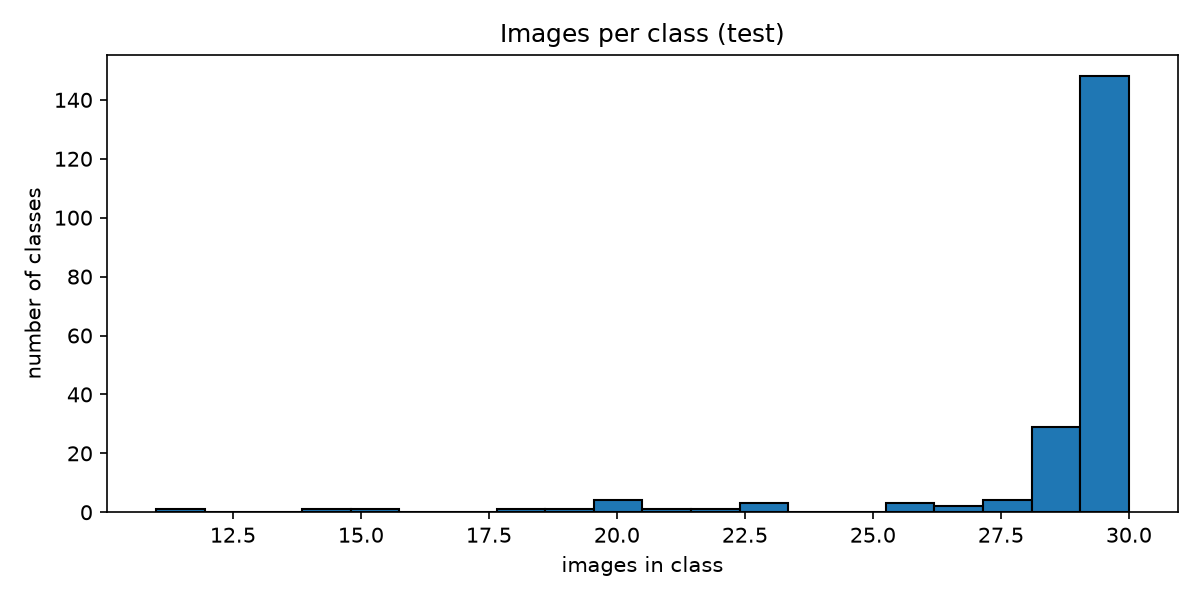
\includegraphics[width=\linewidth]{class_dist_test.png}
\end{subfigure}
\caption{Number of images per class (histogram over the 200 classes).}
\label{fig:classdist}
\end{figure}

\subsection{Image sizes and quality}

Images are at most 500 pixels on their longer side; the median is
500$\times$375 (aspect ratio 1.33), and the smallest is about 120 pixels on
each side (Figure~\ref{fig:imgstats}). Since the models use 128 or 224 pixel
crops, every image has enough resolution. All 11,788 images decode without
errors. Eight images (four per split) are grayscale; the dataset class converts
every image to RGB, which handles them without dropping data.

We also measured brightness, contrast and sharpness (variance of the Laplacian)
for every image (Figure~\ref{fig:quality}). The distributions are wide but
contain no unusable outliers. The eight ``blurriest'' images
(Figure~\ref{fig:blur}) are birds in flight or slightly out of focus, but
several are sharp birds against plain sky or water: the Laplacian measures
texture, so smooth backgrounds also score as blurry. All of these are realistic
inputs, so we keep them.

\begin{figure}[H]
\centering
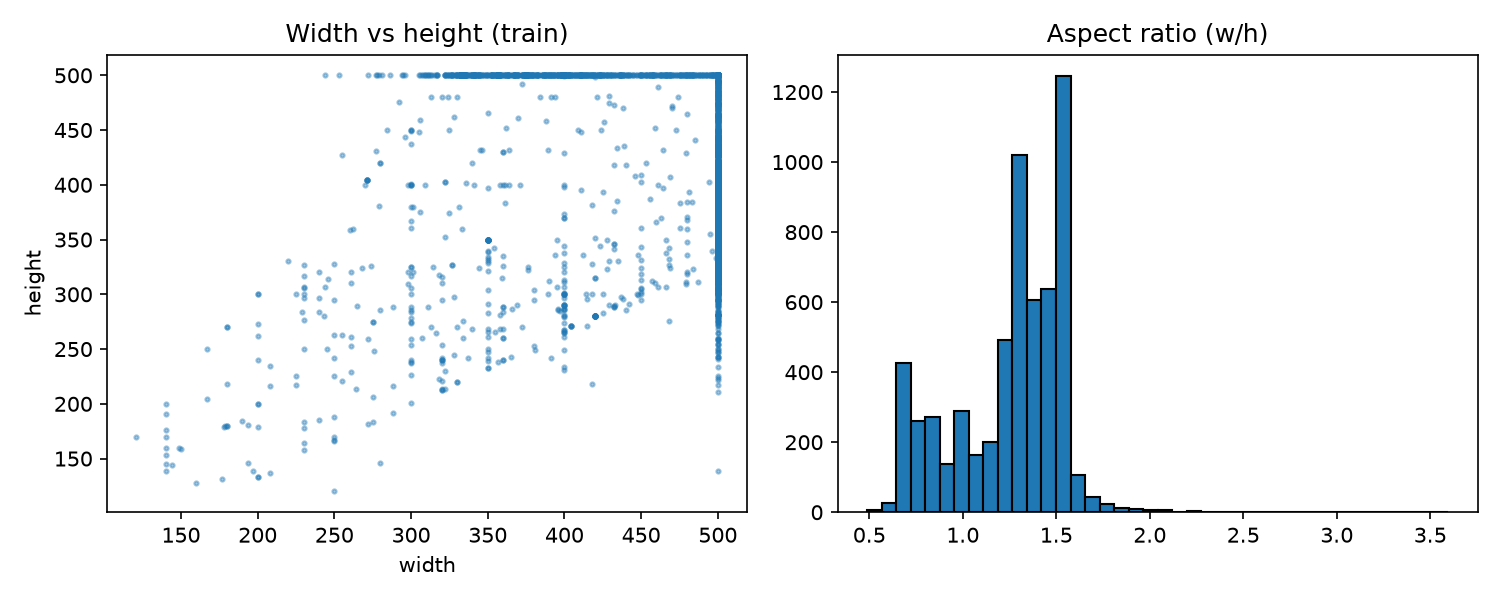
\includegraphics[width=0.75\linewidth]{image_stats_train.png}
\caption{Image width vs.\ height and aspect ratio (train).}
\label{fig:imgstats}
\end{figure}

\begin{figure}[H]
\centering
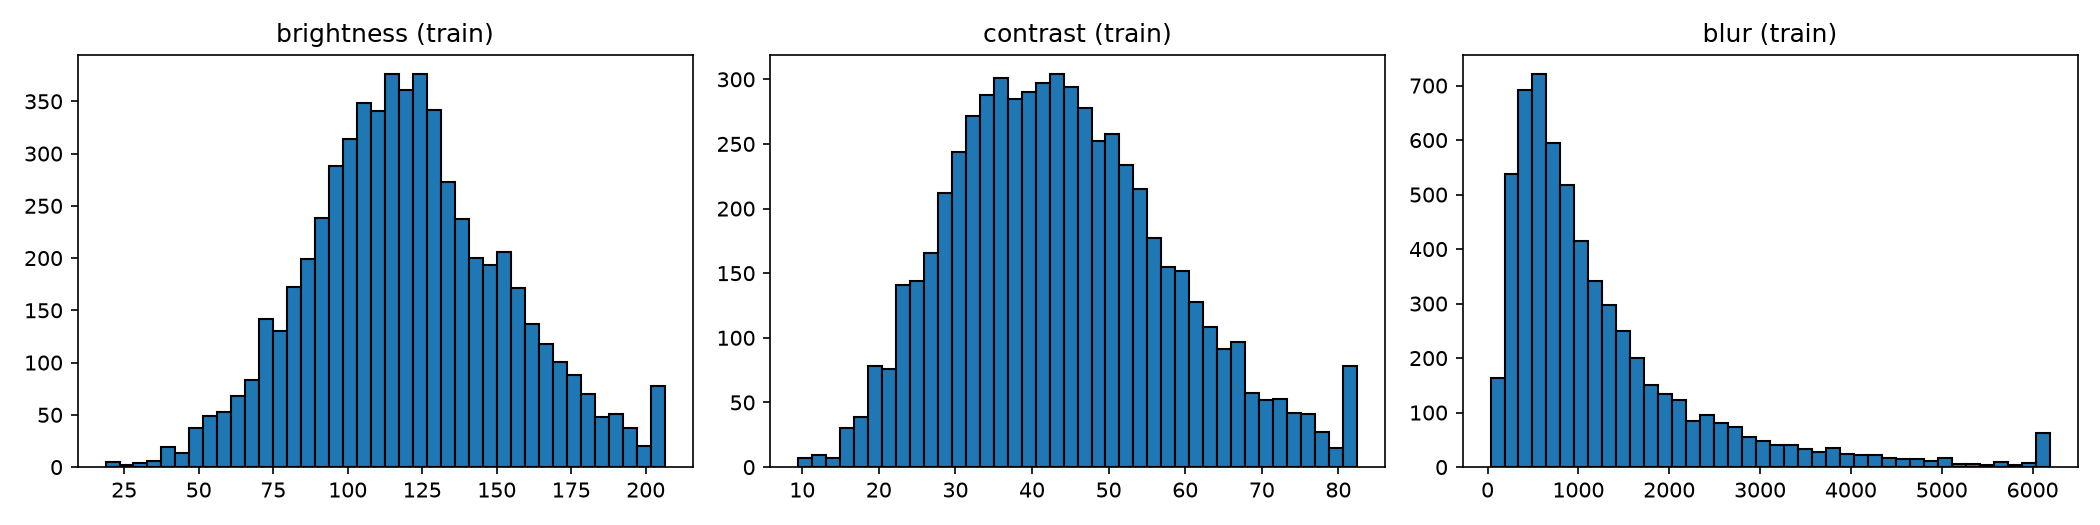
\includegraphics[width=\linewidth]{quality_train.png}
\caption{Brightness, contrast and blur (Laplacian variance) of the training
images; the last bin of each histogram collects values above the 99th
percentile.}
\label{fig:quality}
\end{figure}

\begin{figure}[H]
\centering
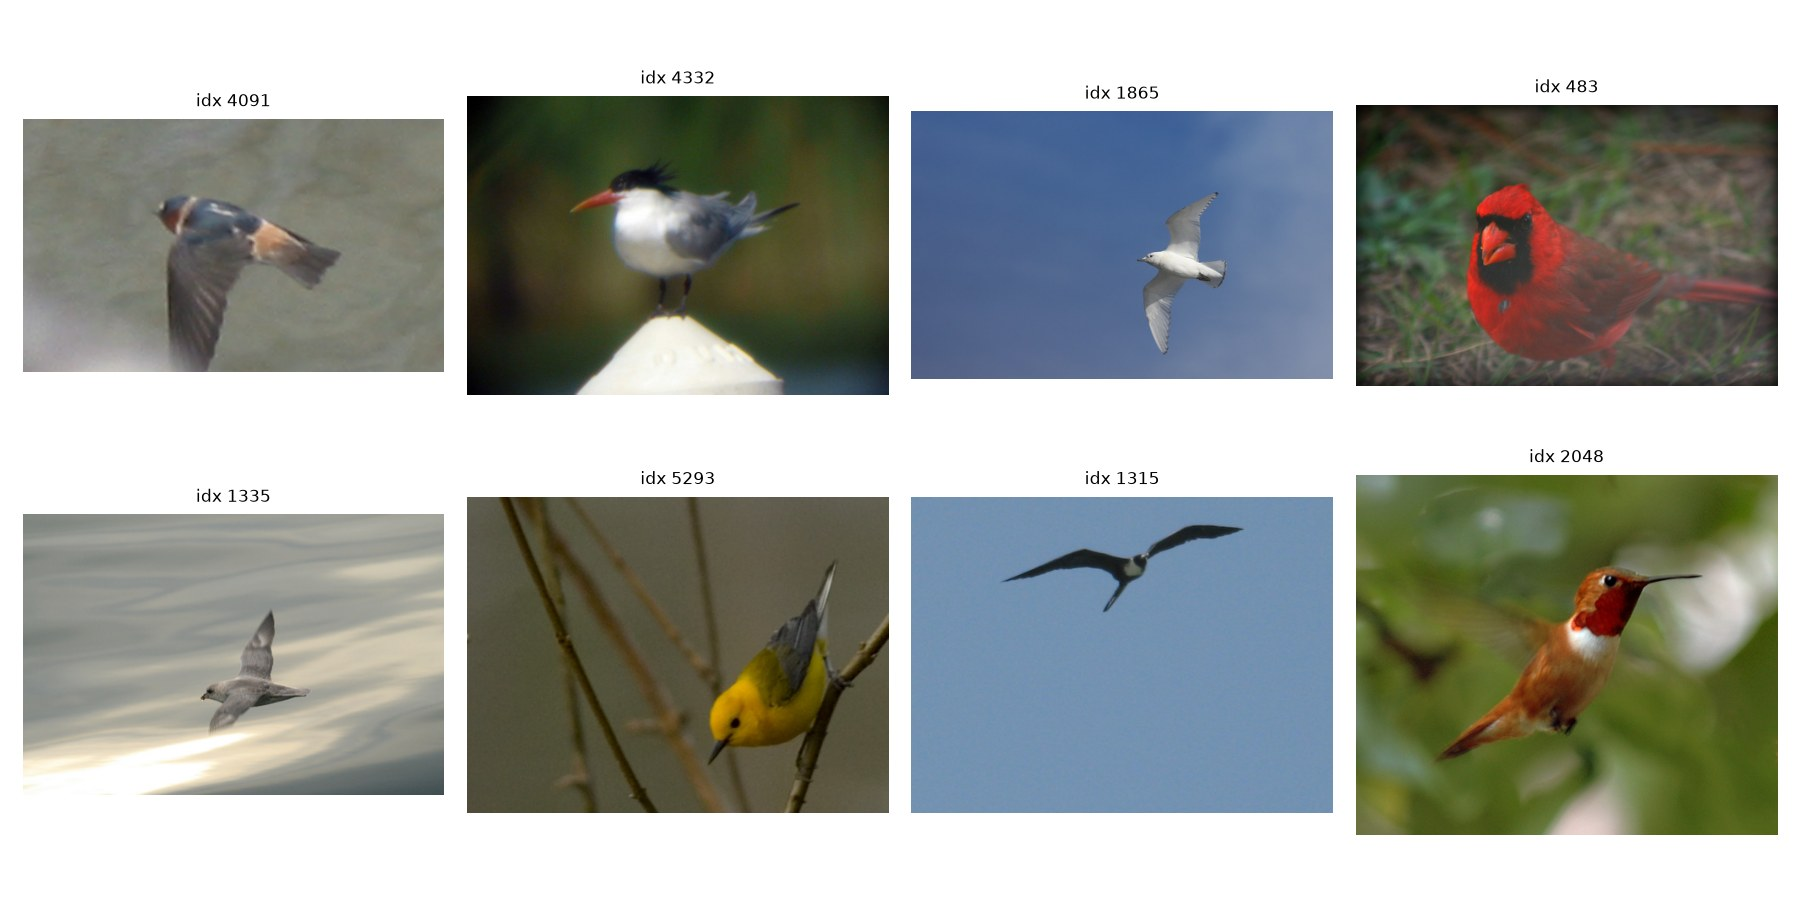
\includegraphics[width=0.75\linewidth]{blurriest_train.jpg}
\caption{The eight blurriest training images.}
\label{fig:blur}
\end{figure}

\subsection{Duplicates and train/test leakage}

We hashed every image twice: an exact MD5 hash of the pixels and a 64-bit
perceptual difference hash (dHash) that survives resizing and re-compression.
We found one near-duplicate pair across the splits: test image 661 matches
training image 774. We confirmed it visually and removed the test image, so the
test set we report on has \textbf{5,793} images. Leaving it in would leak a
training image into the test score.

\subsection{Caption analysis}

The \texttt{description} field holds the ten captions of an image as one string
separated by newlines. Our findings on the training split (59,940 captions):
\begin{itemize}
  \item Every image has exactly ten captions.
  \item Captions are short: 15.2 words on average, 95\% have at most 24 words
        (Figure~\ref{fig:caplen}). A few outliers are 1--2 words long (27
        captions) or longer than 40 words (106 captions).
  \item The raw vocabulary has 4,077 words, of which 1,875 occur only once.
        Many of these rare words are typos: 989 rare words have a close match
        among the common words (e.g.\ \emph{agrayish} vs.\ \emph{grayish}).
  \item 27 captions contain non-ASCII characters (mostly typographic quotes and
        accents).
  \item 9,463 captions are exact duplicates of another caption, such as
        generic descriptions (``this bird is black'') written for several
        birds.
  \item After function words, the most frequent words are colours and body
        parts (\emph{black}, \emph{white}, \emph{brown}, \emph{beak},
        \emph{belly}, \emph{wings}, \emph{yellow}; Figure~\ref{fig:topwords}),
        which shows that captions describe exactly the visual cues a classifier
        needs.
\end{itemize}

\begin{figure}[H]
\centering
\begin{subfigure}{0.49\linewidth}
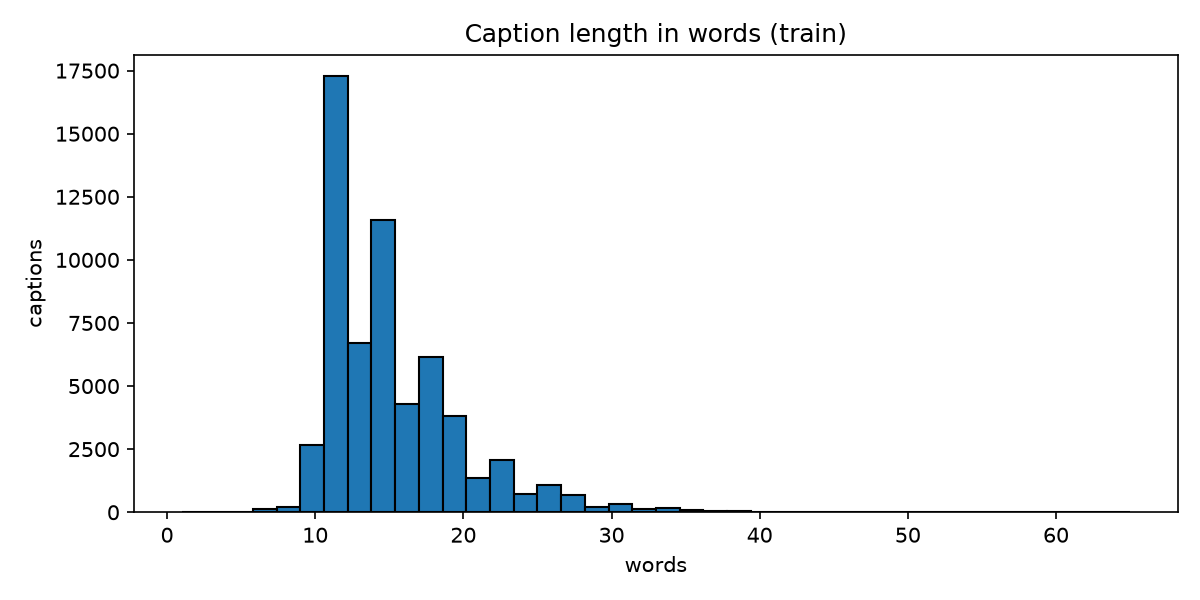
\includegraphics[width=\linewidth]{caption_len_train.png}
\caption{Caption length in words.}
\label{fig:caplen}
\end{subfigure}
\begin{subfigure}{0.49\linewidth}
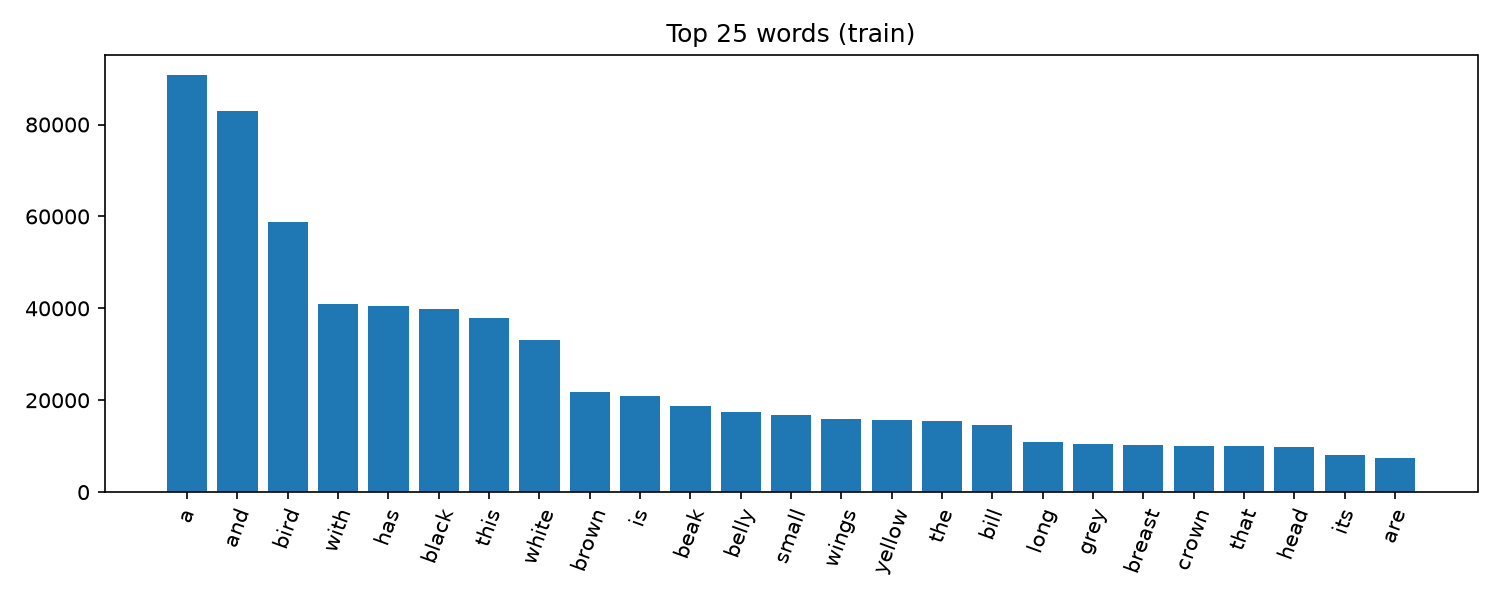
\includegraphics[width=\linewidth]{top_words_train.png}
\caption{Most frequent words.}
\label{fig:topwords}
\end{subfigure}
\caption{Caption statistics (train).}
\end{figure}

\subsection{Caption cleaning}

Captions are cleaned in \texttt{src/data/preprocessing.py} and
\texttt{src/data/captions.py}:
\begin{enumerate}
  \item Split the description on newlines into ten captions.
  \item Replace non-ASCII characters with spaces (replacing instead of deleting
        avoids gluing two words together), lower-case, keep only letters,
        digits and basic punctuation, collapse repeated whitespace.
  \item Drop captions shorter than 3 or longer than 40 words: they are either
        uninformative or rambling outliers. This removes 111 of 59,940
        training captions (0.19\%).
  \item Tokenize into words and build the vocabulary on the \emph{training
        split only} (no validation or test words), keeping words seen at least
        5 times. Rarer words, mostly typos, map to \texttt{<unk>}.
\end{enumerate}
The resulting vocabulary has 1,127 tokens (including \texttt{<pad>},
\texttt{<start>}, \texttt{<end>}, \texttt{<unk>}), and only 0.53\% of training
words become \texttt{<unk>}. Exact duplicate captions are kept: each one is a
valid description of its own image. The captions are used in Milestone~2.

\subsection{Train / validation / test split}

The official training split is divided into training (80\%) and validation
(20\%) with a stratified split (scikit-learn, seed 42), so every species keeps
its proportion: \textbf{4,795 training and 1,199 validation images}. The
validation set chooses the best epoch and the hyperparameters; the test set
(5,793 images) is used only once per final model. A fingerprint of the
validation indices is printed by \texttt{python -m src.check\_env} so all team
members can confirm they use identical splits.

\subsection{Normalization and augmentation}

Images are normalized with the ImageNet mean and standard deviation. The
pretrained ResNet requires these statistics, and we use the same ones for the
scratch model so both see identical inputs.

The training augmentation (\texttt{src/data/transforms.py},
Figure~\ref{fig:aug}) is designed around what does \emph{not} change a bird's
species:
\begin{itemize}
  \item \textbf{RandomResizedCrop} (scale 0.6--1.0): birds appear at different
        sizes and positions; the minimum scale of 0.6 keeps most of the bird
        in view so the label stays correct.
  \item \textbf{Horizontal flip}: a bird facing left is the same species.
        Vertical flips and large rotations are not used because birds are
        almost always upright.
  \item \textbf{Colour jitter} on brightness and contrast (0.2) and a little
        saturation (0.1): covers different lighting. \textbf{Hue is not
        changed}, because colour is one of the most important cues for
        telling species apart (e.g.\ Blue Grosbeak vs.\ Indigo Bunting).
\end{itemize}
Validation and test images are resized to 1.15$\times$ the crop size and
centre-cropped, with no randomness.

\begin{figure}[H]
\centering
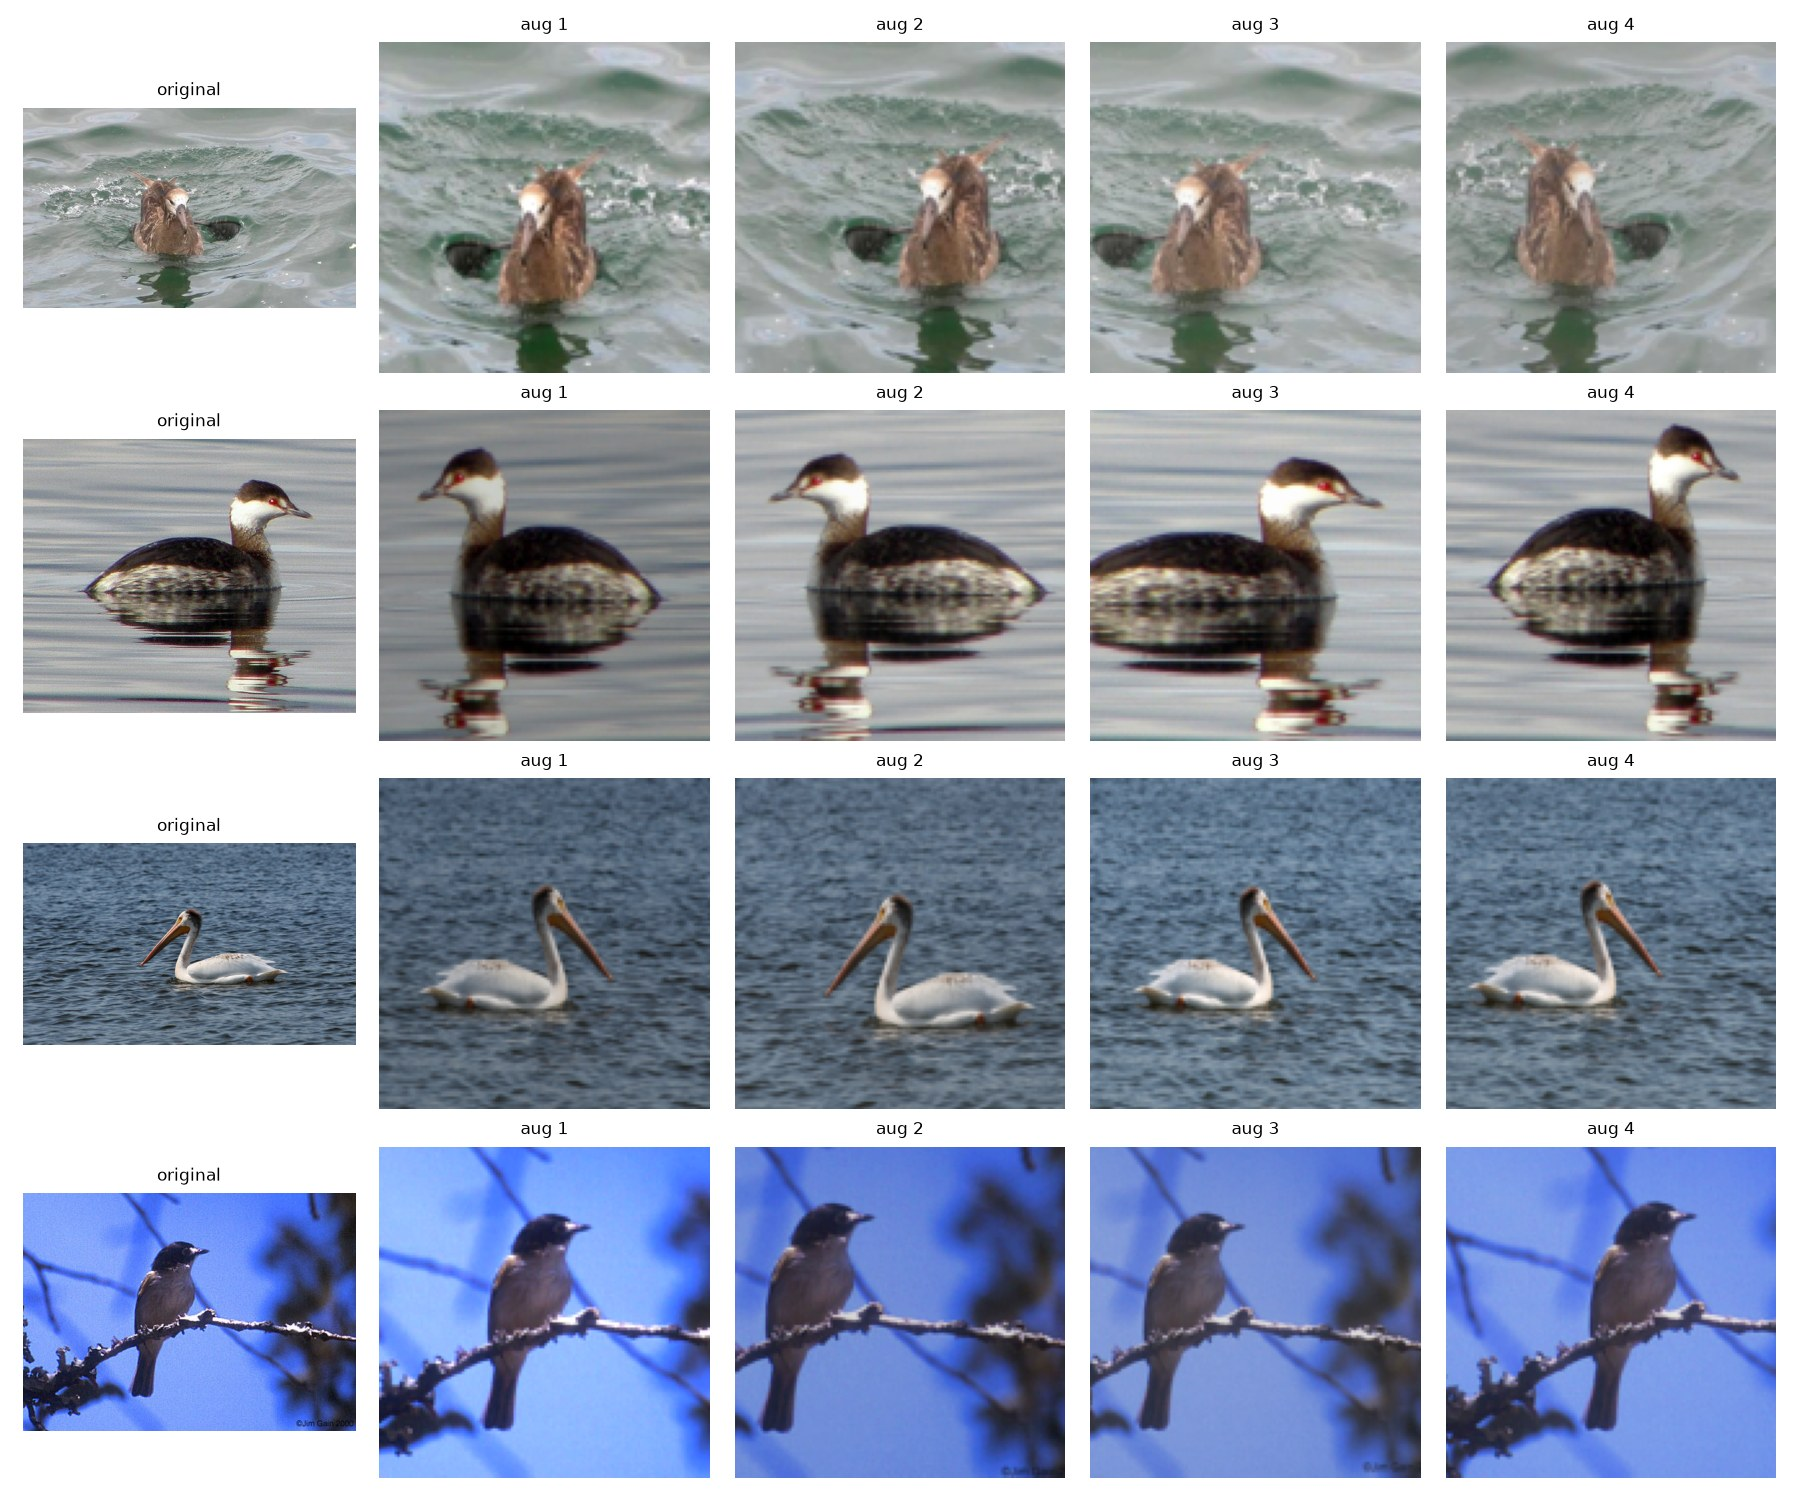
\includegraphics[width=0.8\linewidth]{augmentation_examples.jpg}
\caption{Four random augmentations of each of four training images.}
\label{fig:aug}
\end{figure}

%=====================================================================
\section{Models}
%=====================================================================

All models share one structure: an \emph{encoder} that turns an image into a
spatial feature map, followed by a classification \emph{head} (global average
pooling, dropout 0.3, and a linear layer to 200 classes). The encoder is the
part that Milestone~2 reuses for colorization (as the downsampling half of a
U-Net) and captioning (frozen features fed to a decoder).

\subsection{CNN from scratch (baseline)}

The scratch encoder (\texttt{src/models/scratch\_cnn.py}) has five blocks.
Each block is two 3$\times$3 convolutions, each followed by batch
normalization~\cite{ioffe2015} and ReLU, then 2$\times$2 max pooling. The
channel widths are 32, 64, 128, 256 and 512, so a 128$\times$128 image becomes
a 512$\times$4$\times$4 feature map. The whole classifier has 4.82\,M
parameters, all randomly initialised. We use 128-pixel inputs to keep training
fast; this is a deliberate trade-off against detail.

\subsection{ResNet-18 transfer learning}

The transfer encoder (\texttt{src/models/pretrained.py}) is a
ResNet-18~\cite{he2016} with ImageNet weights~\cite{deng2009}
(\texttt{IMAGENET1K\_V1} from torchvision), without its average pooling and
1000-class layer. With 224-pixel inputs it produces a 512$\times$7$\times$7
feature map. It exposes the same interface as the scratch encoder, so the same
head, trainer and Grad-CAM code work unchanged. We use it in two ways:
\begin{itemize}
  \item \textbf{Frozen (feature extraction):} the encoder weights are fixed
        and only the head trains (102,600 parameters). Batch-normalization
        statistics are frozen too, so the pretrained features do not drift.
  \item \textbf{Fine-tuned:} all 11.28\,M parameters train. The pretrained
        encoder uses a 10$\times$ smaller learning rate (0.0001) than the new
        head (0.001), so it adapts to birds without losing its ImageNet
        features.
\end{itemize}

\subsection{Training setup}

All models are implemented in PyTorch~\cite{pytorch} and trained by the same
loop (\texttt{src/training/trainer.py}):
AdamW~\cite{loshchilov2019}, a cosine learning-rate schedule~\cite{loshchilov2017}
down to zero over the run, cross-entropy with label smoothing
0.1~\cite{szegedy2016}, and mixed precision on the GPU. After every epoch the
model is evaluated on the validation set, and the checkpoint with the best
validation accuracy is kept. All runs use seed 42 and were trained on a Kaggle
NVIDIA T4 GPU. Configurations are YAML files in \texttt{configs/}.

\begin{table}[H]
\centering
\caption{Training configurations of the final models.}
\label{tab:configs}
\resizebox{\linewidth}{!}{%
\begin{tabular}{lcccccc}
\toprule
Model & Input & Batch & LR (head / encoder) & Weight decay & Epochs & Trainable params \\
\midrule
Scratch CNN (tuned) & 128 & 64 & 0.0003 / 0.0003 & 0.005 & 60 & 4.82\,M \\
ResNet-18 frozen & 224 & 32 & 0.001 / --- & 0.0001 & 15 & 0.10\,M \\
ResNet-18 fine-tuned & 224 & 32 & 0.001 / 0.0001 & 0.0001 & 15 & 11.28\,M \\
\bottomrule
\end{tabular}}
\end{table}

%=====================================================================
\section{Experiments}
%=====================================================================

Table~\ref{tab:runs} lists every classification run, and
Figure~\ref{fig:valcurves} compares their validation curves.

\begin{table}[H]
\centering
\caption{Classification runs. ``Gap'' is training minus validation accuracy at
the best epoch; training accuracy is measured on augmented images.}
\label{tab:runs}
\resizebox{\linewidth}{!}{%
\begin{tabular}{lccccccc}
\toprule
Run & Best epoch & Val acc. & Val top-5 & Val F1 & Train acc. & Gap & Minutes \\
\midrule
Scratch CNN (default) & 29 / 30 & 31.9\% & 62.2\% & 0.306 & 50.4\% & 18.5 & 5.8 \\
Scratch CNN (tuned) & 59 / 60 & 47.4\% & 73.0\% & 0.465 & 96.2\% & 48.8 & 11.6 \\
ResNet-18 frozen & 15 / 15 & 60.7\% & 87.2\% & 0.601 & 77.6\% & 16.9 & 3.9 \\
ResNet-18 fine-tuned & 14 / 15 & 72.4\% & 92.1\% & 0.720 & 99.1\% & 26.7 & 4.1 \\
\bottomrule
\end{tabular}}
\end{table}

\begin{figure}[H]
\centering
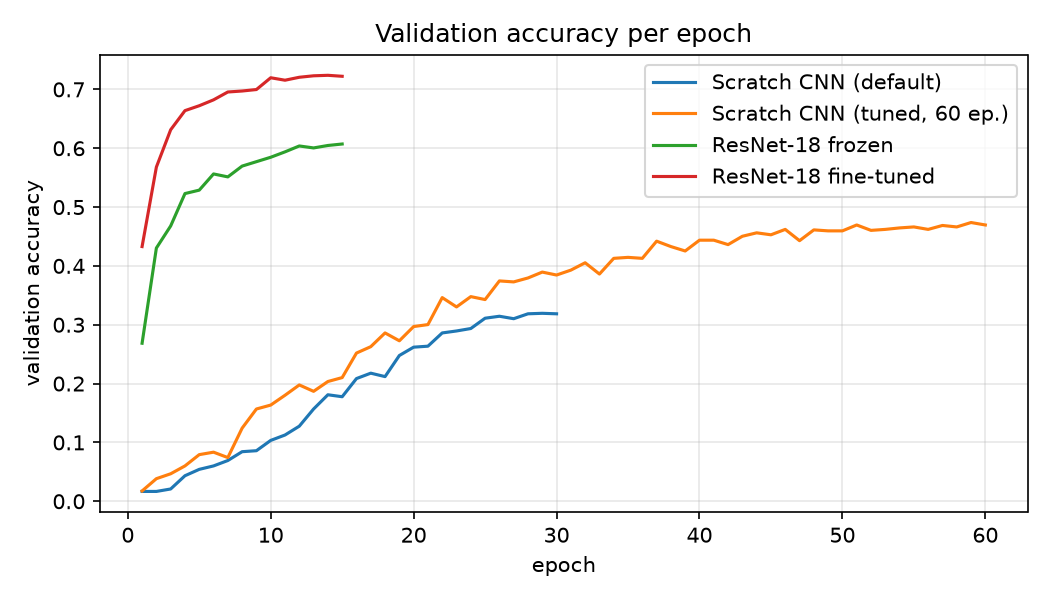
\includegraphics[width=0.8\linewidth]{val_curves_all.png}
\caption{Validation accuracy per epoch of the four classification runs.}
\label{fig:valcurves}
\end{figure}

\subsection{Baseline vs.\ tuned scratch CNN}

The default scratch run (learning rate 0.001, 30 epochs) reached 31.9\%. Its
validation accuracy was still rising when the cosine schedule ended. Tuning
(Section~\ref{sec:tuning}) moved the learning rate to 0.0003, which gave
39.2\% in 30 epochs, and training the tuned model for 60 epochs gave
\textbf{47.4\%}: +15.5 points over the baseline. The longer run converges
(validation accuracy is flat from about epoch 46) but overfits heavily: the
model fits 96\% of the (augmented) training images while validation accuracy
stays at 47\% (Figure~\ref{fig:curves_scratch}). With about 24 training images
per species, the network can memorise the training set.

\subsection{Scratch vs.\ transfer learning}

Transfer learning dominates. After a single epoch, the fine-tuned ResNet-18
(43.3\% validation accuracy) is almost level with the scratch CNN after 60
epochs, and it finishes at 72.4\% in 15 epochs and about 4 minutes.
\begin{itemize}
  \item \textbf{Frozen} features already reach 60.7\% with only a linear head
        trained. ImageNet features locate the bird and its parts well, but they
        are not specialised for distinguishing similar species, so the frozen
        model plateaus (Figure~\ref{fig:curves_resnet}, left).
  \item \textbf{Fine-tuning} lets the encoder adapt to fine-grained details and
        adds 11.7 points. It also memorises the training set (99\% training
        accuracy), but validation loss keeps decreasing, so the overfitting
        does not hurt the validation score.
\end{itemize}

\begin{figure}[H]
\centering
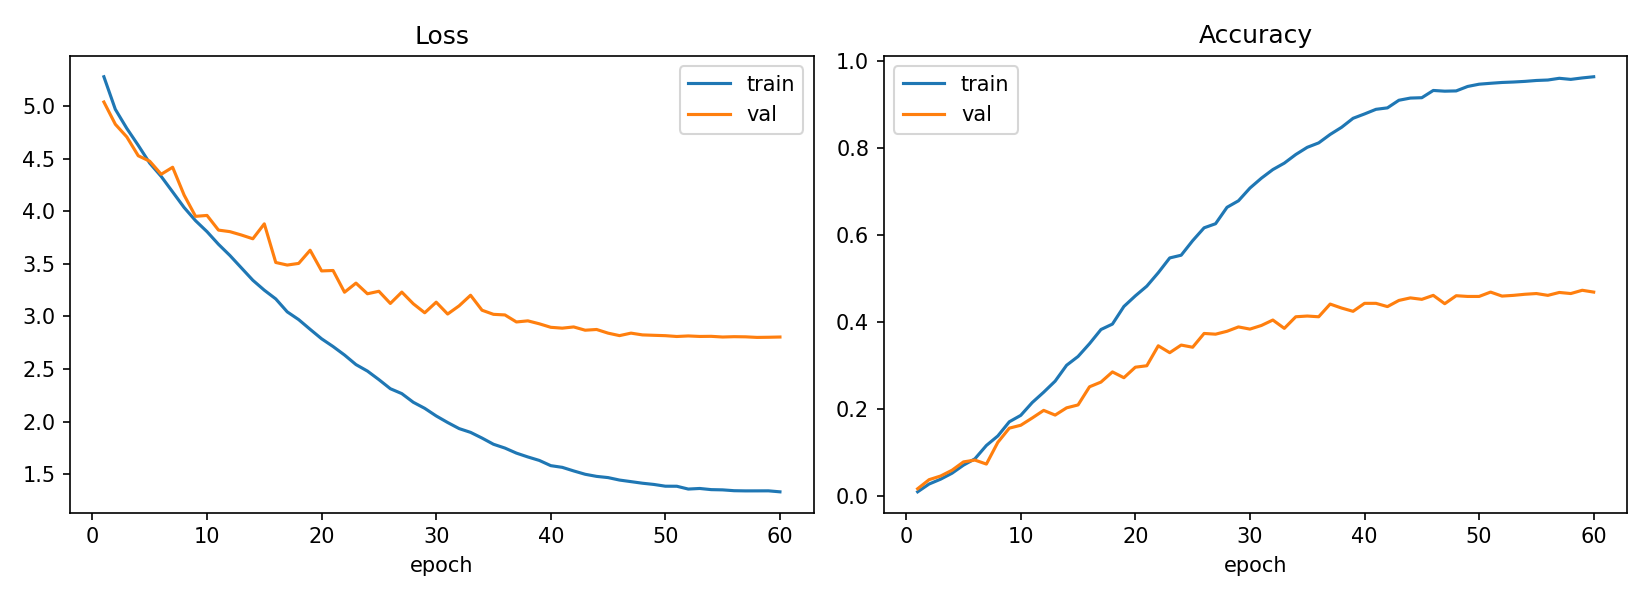
\includegraphics[width=0.75\linewidth]{scratch_tuned_curves.png}
\caption{Training vs.\ validation loss and accuracy, tuned scratch CNN.}
\label{fig:curves_scratch}
\end{figure}

\begin{figure}[H]
\centering
\begin{subfigure}{0.49\linewidth}
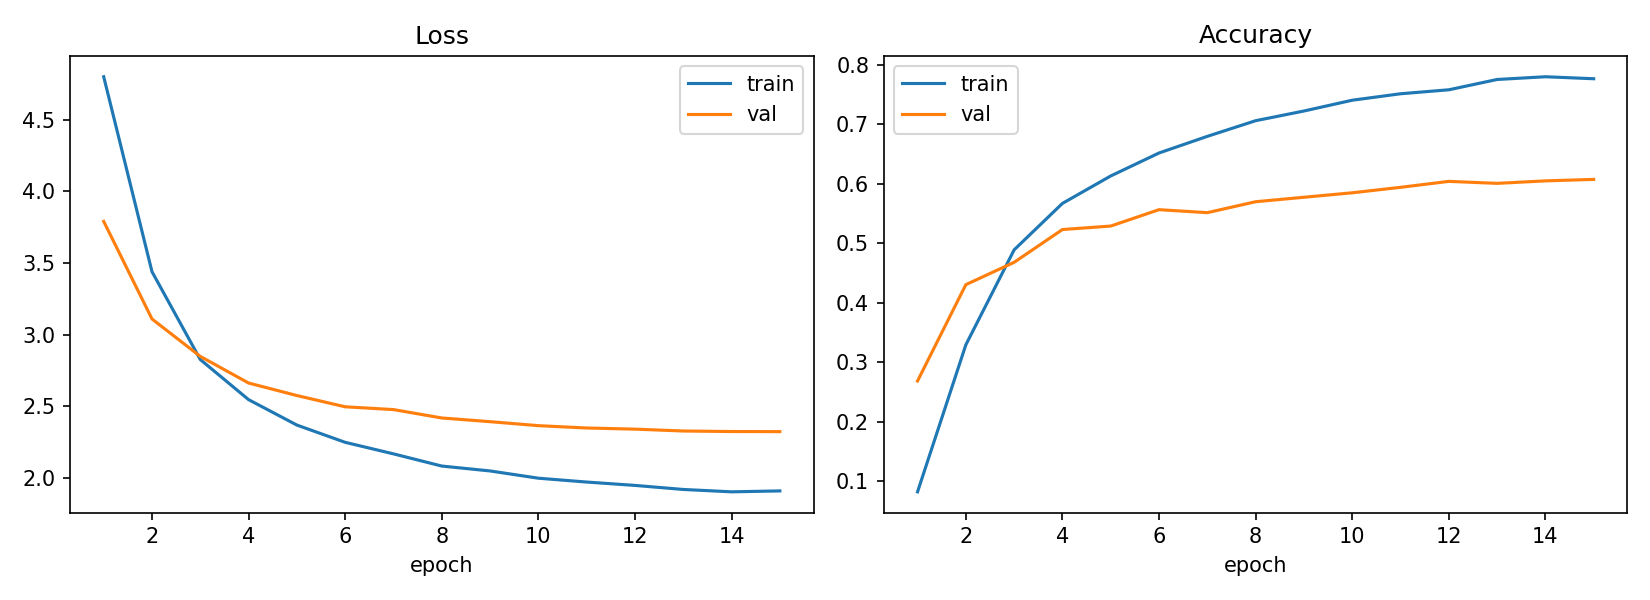
\includegraphics[width=\linewidth]{resnet18_frozen_curves.png}
\caption{Frozen.}
\end{subfigure}
\begin{subfigure}{0.49\linewidth}
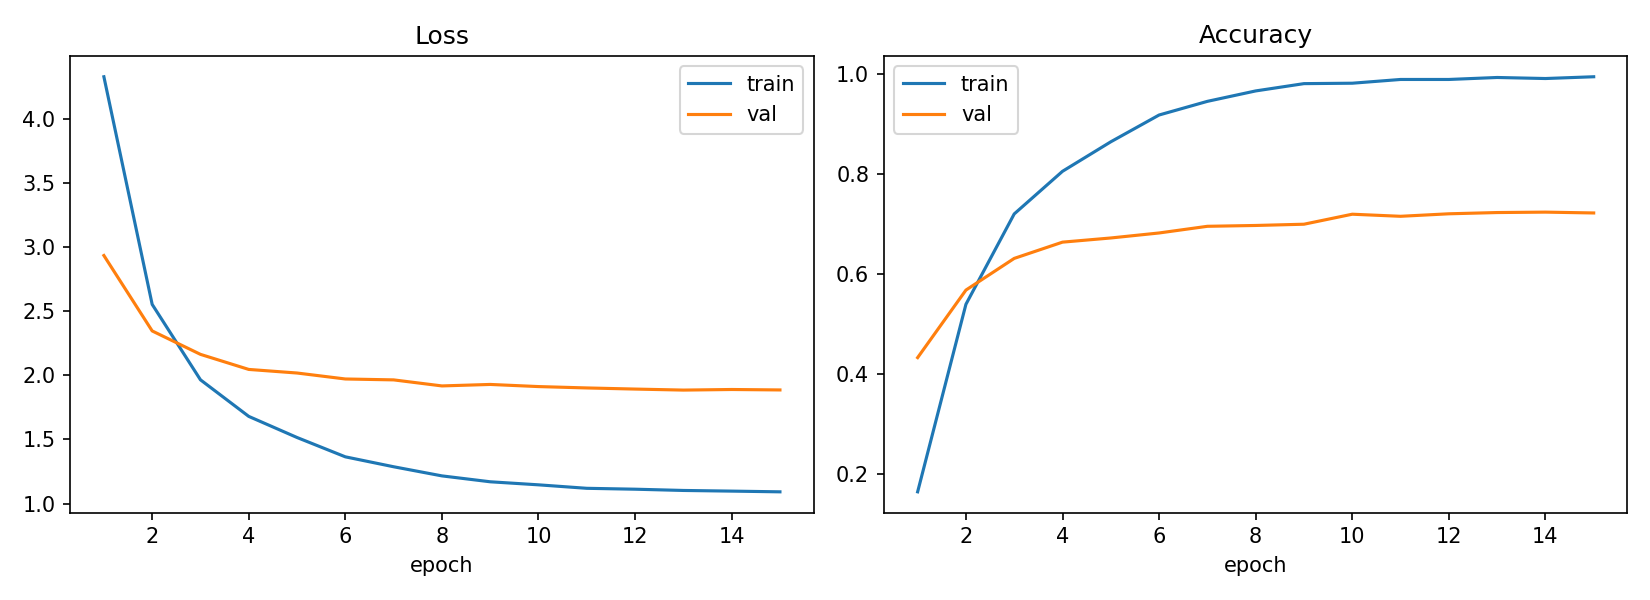
\includegraphics[width=\linewidth]{resnet18_finetune_curves.png}
\caption{Fine-tuned.}
\end{subfigure}
\caption{Training vs.\ validation curves of the ResNet-18 models.}
\label{fig:curves_resnet}
\end{figure}

The loss values in the curves include label smoothing, so they cannot reach
zero: with smoothing 0.1 over 200 classes the lowest possible loss is about
0.85, which is why the fine-tuned model's training loss stops near 1.1.

%=====================================================================
\section{Hyperparameter Tuning}
\label{sec:tuning}
%=====================================================================

Tuning was done on the scratch CNN (\texttt{src/training/tuning.py},
\texttt{python -m src.cli tune}), because it is the model most sensitive to its
settings and is cheap to train (about 6 minutes per 30-epoch trial). Every
trial uses the base configuration with 30 epochs and the same seed, and is
scored by its best validation accuracy.

\paragraph{Search space.} We tuned the learning rate and the weight decay of
AdamW, the two settings that most directly control how fast and how freely the
network fits the small training set.
\begin{itemize}
  \item \textbf{Grid search:} learning rate $\in \{0.0003, 0.001, 0.003\}$
        $\times$ weight decay $\in \{0.0005, 0.005, 0.05\}$, 9 trials.
  \item \textbf{Random search~\cite{bergstra2012}:} 9 trials, both parameters
        drawn log-uniformly from the same ranges (0.0003--0.003 and
        0.0005--0.05), seed 0.
\end{itemize}
Both methods get the same budget and the same bounds, so the comparison is fair.

\begin{table}[H]
\centering
\caption{Grid search: best validation accuracy of each trial.}
\label{tab:grid}
\begin{tabular}{lccc}
\toprule
Learning rate $\backslash$ weight decay & 0.0005 & 0.005 & 0.05 \\
\midrule
0.0003 & 38.3\% & \textbf{39.2\%} & 38.9\% \\
0.001 & 31.9\% & 34.4\% & 33.9\% \\
0.003 & 28.4\% & 26.6\% & 28.3\% \\
\bottomrule
\end{tabular}
\end{table}

\begin{table}[H]
\centering
\caption{Random search trials, in the order they were run.}
\label{tab:random}
\begin{tabular}{lccccccccc}
\toprule
Trial & 1 & 2 & 3 & 4 & 5 & 6 & 7 & 8 & 9 \\
\midrule
LR ($\times 10^{-3}$) & 2.10 & 0.79 & 0.97 & 1.82 & 0.90 & 2.43 & 0.57 & 1.25 & 2.44 \\
WD ($\times 10^{-3}$) & 16.4 & 1.6 & 3.2 & 2.0 & 7.3 & 5.1 & 16.2 & 1.6 & 46.2 \\
Val acc. (\%) & 29.5 & 33.5 & 33.4 & 31.9 & 33.1 & 29.8 & \textbf{35.6} & 32.6 & 31.9 \\
\bottomrule
\end{tabular}
\end{table}

\begin{table}[H]
\centering
\caption{Grid search vs.\ random search (\texttt{outputs/tuning/comparison.csv}).}
\label{tab:tunecompare}
\resizebox{\linewidth}{!}{%
\begin{tabular}{lcccccc}
\toprule
Method & Trials & Best val acc. & Best found at & Minutes to best & Total minutes & Mean val acc. \\
\midrule
Grid & 9 & \textbf{39.2\%} & 2nd trial & \textbf{11.8} & 53.0 & 33.3\% \\
Random & 9 & 35.6\% & 7th trial & 40.4 & 52.2 & 32.4\% \\
\bottomrule
\end{tabular}}
\end{table}

\begin{figure}[H]
\centering
\begin{subfigure}{0.49\linewidth}
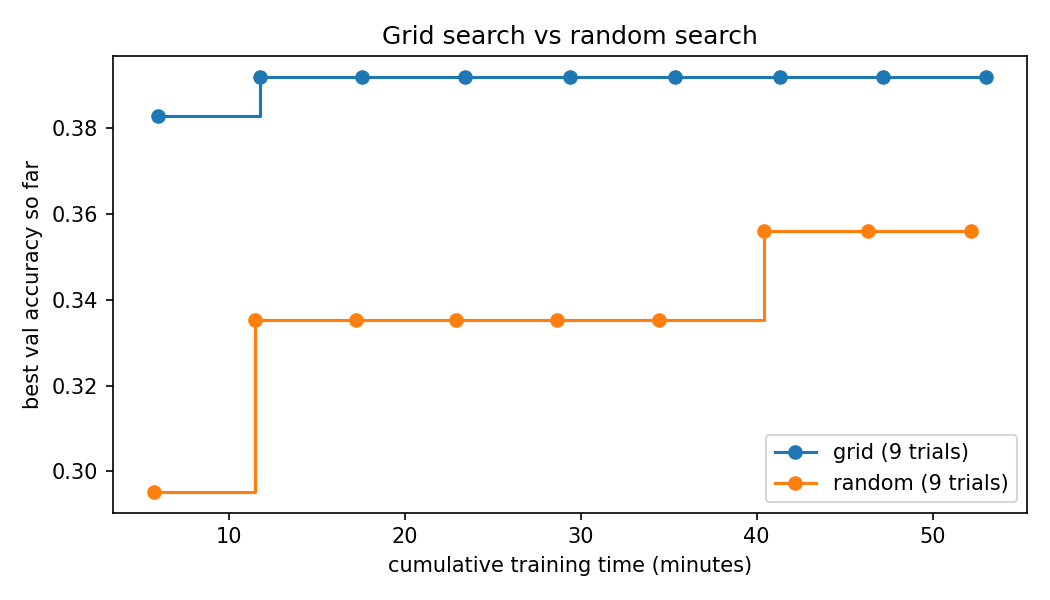
\includegraphics[width=\linewidth]{tuning_best_so_far.png}
\caption{Best accuracy found vs.\ time spent.}
\end{subfigure}
\begin{subfigure}{0.42\linewidth}
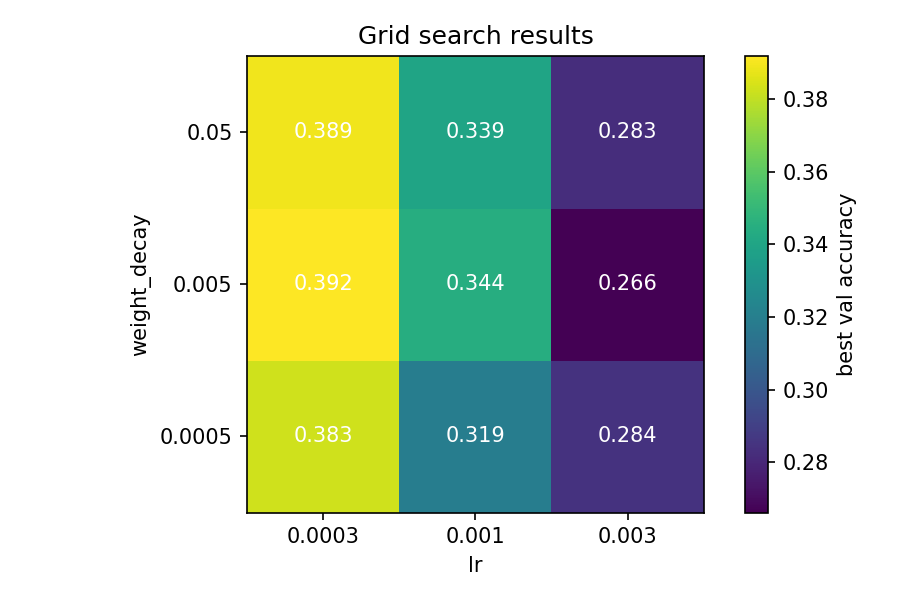
\includegraphics[width=\linewidth]{grid_heatmap.png}
\caption{Grid search results.}
\end{subfigure}
\caption{Hyperparameter tuning results.}
\label{fig:tuning}
\end{figure}

\paragraph{Findings.}
\begin{itemize}
  \item \textbf{The learning rate dominates.} Each row of the grid is clearly
        separated (about 39\%, 34\% and 28\%), and in both searches accuracy
        rises steadily as the learning rate falls.
  \item \textbf{Weight decay barely matters.} Within a row, values differ by
        1--3 points, which is close to the noise level of the validation set
        (about $\pm$1.4 points for 1,199 images).
  \item \textbf{Grid search won here}, both in best score (39.2\% vs.\ 35.6\%)
        and in speed (best result after 11.8 instead of 40.4 minutes). Random
        search is usually better when several hyperparameters matter, because
        it tries more distinct values of each one~\cite{bergstra2012}. Here only
        one parameter matters, and its best value lies exactly on the lowest
        grid point; random search, by chance, drew no learning rate below
        0.00057, and its best trial was exactly its lowest learning rate.
\end{itemize}

\paragraph{Coarse-to-fine follow-up.} Because the best learning rate lay on the
edge of the range, we ran a second grid below it with weight decay fixed at
0.005: learning rate 0.0001 gave 30.4\%, 0.00015 gave 36.4\% and 0.0002 gave
37.9\%. Accuracy therefore peaks at 0.0003 and falls on both sides, confirming
it as the optimum rather than an artefact of the range. The lowest learning
rates were not unstable but too slow: they had not converged within 30 epochs.

\paragraph{Final choice.} Learning rate 0.0003 and weight decay 0.005, trained
for 60 instead of 30 epochs because the best tuning trials were still improving
at epoch 30. Hyperparameter tuning was required for Milestone~1 only; the
ResNet models use standard fine-tuning settings.

%=====================================================================
\section{Experiment Tracking}
%=====================================================================

Every run is logged to MLflow~\cite{mlflow} (SQLite backend,
\texttt{mlflow.db}): all hyperparameters, the device, the total and trainable
parameter counts, per-epoch training and validation loss, accuracy, macro
precision, recall, F1 and top-5 accuracy, the learning rate, the training-curve
plot, and the best checkpoint. Classification runs are in the experiment
\texttt{classification} (4 runs) and the 21 tuning trials in
\texttt{tuning\_scratch}, each tagged with its search method. Any run can be
opened with \texttt{mlflow ui --backend-store-uri sqlite:///mlflow.db}.
Tables~\ref{tab:runs}--\ref{tab:random} and Figure~\ref{fig:valcurves} are
exported from these runs.

\begin{figure}[H]
\centering
\IfFileExists{figures/mlflow_ui.png}{%
  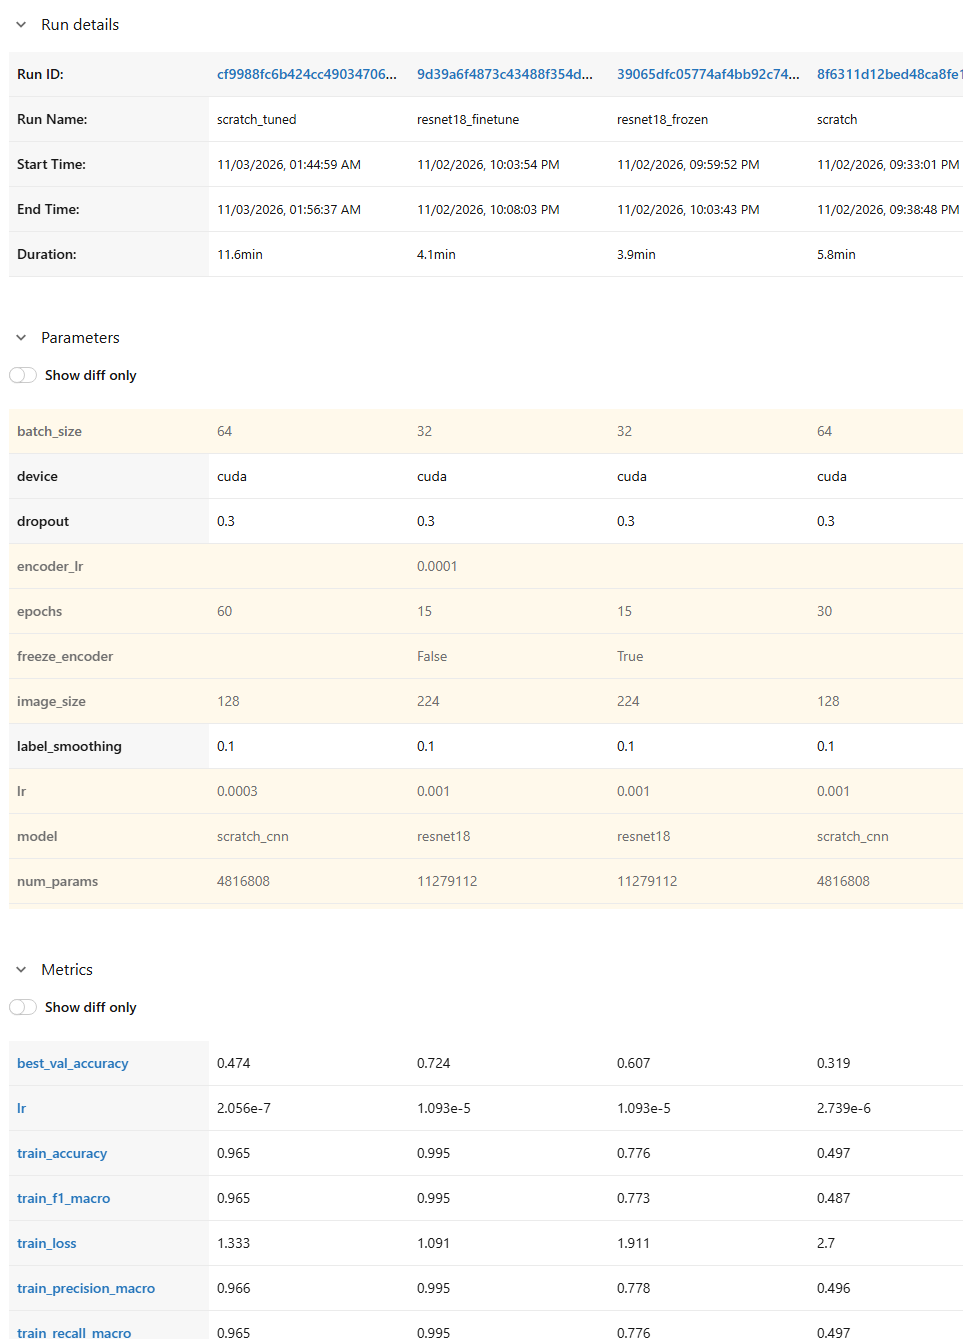
\includegraphics[width=\linewidth]{mlflow_ui.png}%
}{%
  \fbox{\parbox{0.9\linewidth}{\centering\vspace{1.5cm}
  \todo{add a screenshot of the MLflow UI comparing the classification runs
  as figures/mlflow\_ui.png}\vspace{1.5cm}}}%
}
\caption{MLflow: comparison of the classification runs.}
\label{fig:mlflow}
\end{figure}

%=====================================================================
\section{Evaluation}
%=====================================================================

\subsection{Metrics}

With $TP_c$, $FP_c$ and $FN_c$ the true positives, false positives and false
negatives of class $c$, and $C = 200$ classes:
\begin{itemize}
  \item \textbf{Accuracy} --- the fraction of images whose top prediction is
        the correct species. It answers ``how often is the model right?''.
  \item \textbf{Macro precision} $\frac{1}{C}\sum_c \frac{TP_c}{TP_c+FP_c}$ ---
        when the model predicts a species, how often it is correct, averaged
        so every species counts equally.
  \item \textbf{Macro recall} $\frac{1}{C}\sum_c \frac{TP_c}{TP_c+FN_c}$ --- of
        the images of a species, how many the model finds.
  \item \textbf{Macro F1} --- the average over classes of the harmonic mean of
        precision and recall. It is low if a model ignores some classes, even
        when overall accuracy looks good.
  \item \textbf{Top-5 accuracy} --- the fraction of images whose correct
        species is among the five highest-scoring predictions. For
        fine-grained data it shows whether errors are ``near misses''
        between similar species.
  \item \textbf{Confusion matrix} --- counts of true vs.\ predicted class; it
        shows which species are confused with each other.
\end{itemize}

\subsection{Test results}

\begin{table}[H]
\centering
\caption{Final models on the test set (5,793 images, evaluated once each with
\texttt{python -m src.cli evaluate}). Full table:
\texttt{outputs/eval/model\_comparison.csv}.}
\label{tab:test}
\begin{tabular}{lcccccc}
\toprule
Model & Val acc. & Test acc. & Precision & Recall & F1 & Top-5 \\
\midrule
Scratch CNN (tuned) & 47.4\% & 49.6\% & 0.504 & 0.499 & 0.495 & 76.6\% \\
ResNet-18 frozen & 60.7\% & 64.3\% & 0.649 & 0.647 & 0.643 & 89.1\% \\
ResNet-18 fine-tuned & 72.4\% & \textbf{74.4\%} & \textbf{0.751} & \textbf{0.746} & \textbf{0.743} & \textbf{92.3\%} \\
\bottomrule
\end{tabular}
\end{table}

\paragraph{Interpretation.}
\begin{itemize}
  \item \textbf{Ranking.} Fine-tuned $>$ frozen $>$ scratch, by 10.1 and 14.7
        points. The fine-tuned model identifies three out of four birds
        correctly among 200 species; the scratch model one in two, which is
        still about 100 times better than chance (0.5\%).
  \item \textbf{Balance across species.} For every model, macro precision,
        recall and F1 are within about one point of accuracy. No model reaches
        its accuracy by mastering a few easy species and ignoring others.
  \item \textbf{Near misses.} Top-5 accuracy is far above top-1 (92.3\% vs.\
        74.4\% for the fine-tuned model): most errors put the true species
        among the top candidates. Section~\ref{sec:gradcam} shows these are
        mostly confusions between very similar species.
  \item \textbf{Test vs.\ validation.} All three models score 2--4 points
        \emph{higher} on test than on validation. The validation set is small
        (about 6 images per species, $\pm$1.4 points of noise), and all models
        are measured on the same validation images, so a slightly harder
        validation sample lowers all three together. The larger test set is
        the more reliable estimate, and the result also shows that choosing
        the best epoch on validation did not inflate the test scores.
  \item The test loss uses plain cross-entropy, while training and validation
        losses include label smoothing, so the loss values are not comparable
        between them; we compare models by accuracy and F1.
\end{itemize}

\begin{figure}[H]
\centering
\begin{subfigure}{0.49\linewidth}
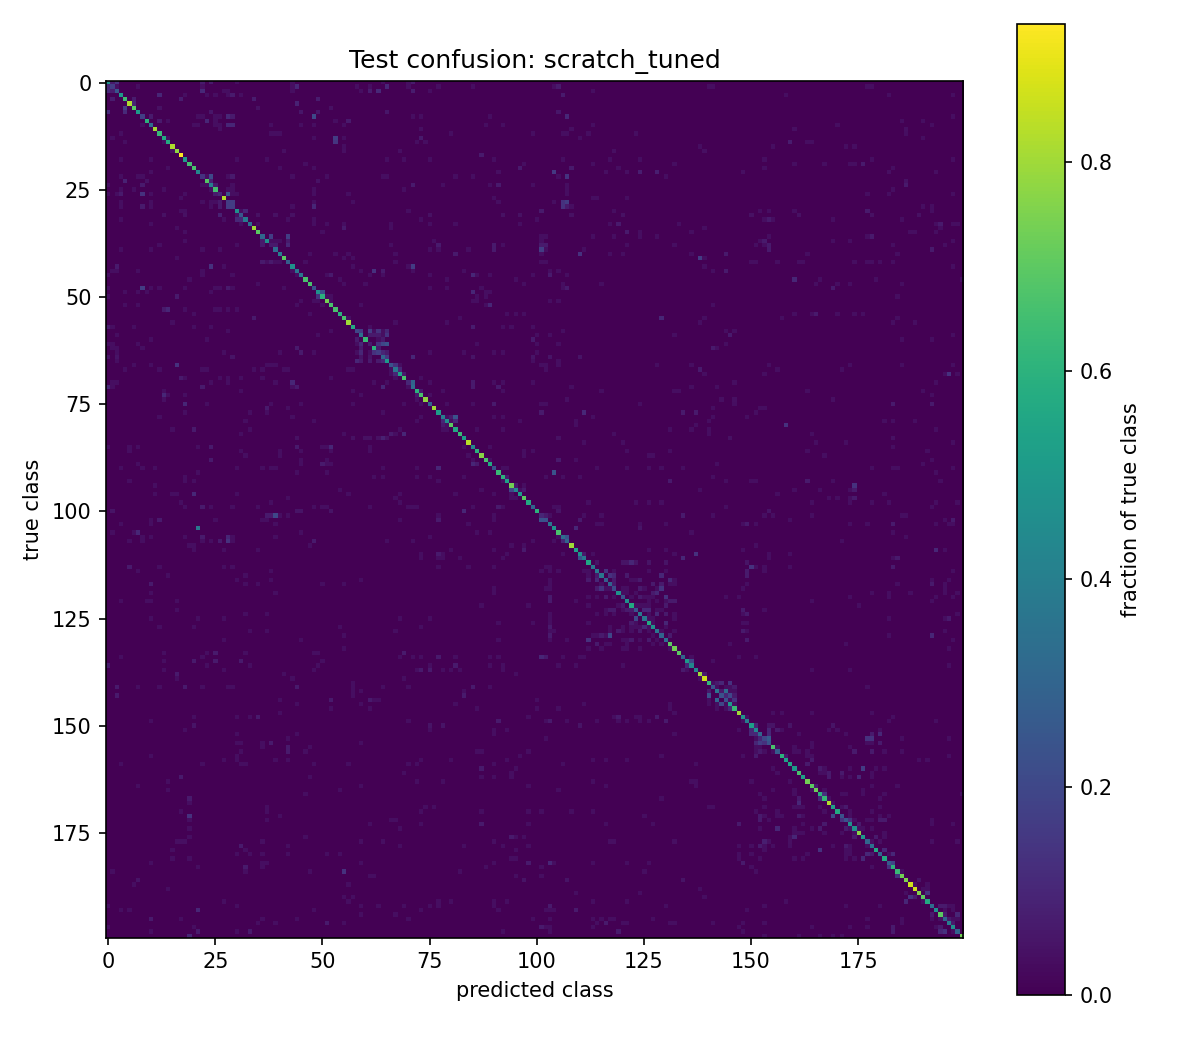
\includegraphics[width=\linewidth]{scratch_tuned_confusion.png}
\caption{Scratch CNN (tuned).}
\end{subfigure}
\begin{subfigure}{0.49\linewidth}
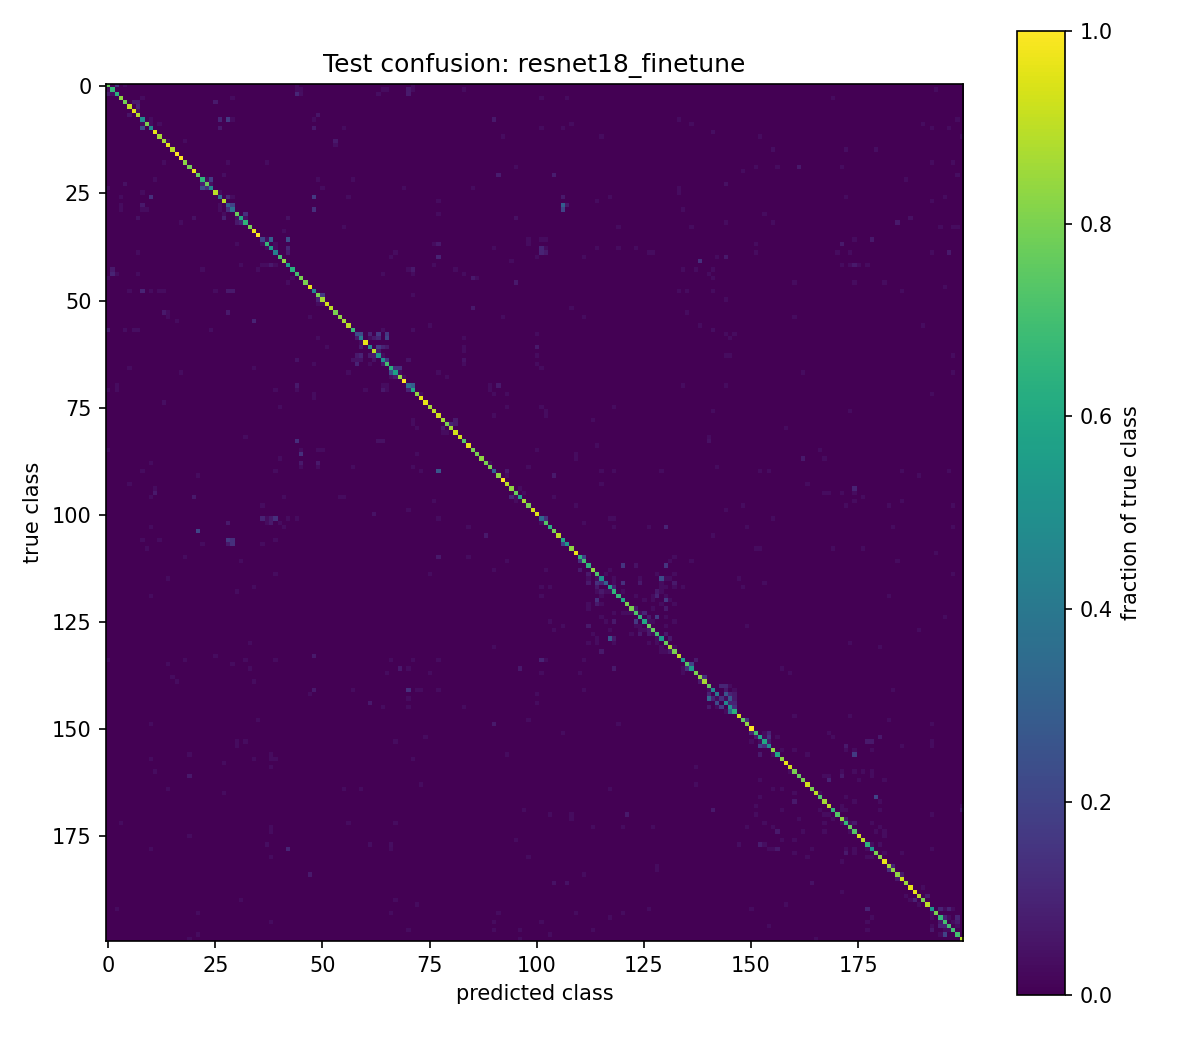
\includegraphics[width=\linewidth]{resnet18_finetune_confusion.png}
\caption{ResNet-18 fine-tuned.}
\end{subfigure}
\caption{Normalized test confusion matrices (200$\times$200; rows are true
classes). The fine-tuned model has a much sharper diagonal. Its errors form
small blocks next to the diagonal: the class list is ordered by family, so
these are confusions within a family, most visibly gulls (classes 58--65),
sparrows (112--132), terns (140--146) and warblers (157--181).}
\label{fig:confusion}
\end{figure}

%=====================================================================
\section{Explainability: Grad-CAM}
\label{sec:gradcam}
%=====================================================================

Grad-CAM~\cite{selvaraju2017} (\texttt{src/visualization/gradcam.py},
\texttt{python -m src.cli explain}) shows which image regions pushed the model
towards a class. For the class score $y^c$ and the feature maps $A^k$ of the
last convolutional stage, each channel gets the weight
$\alpha_k^c = \frac{1}{Z}\sum_{i,j} \partial y^c / \partial A^k_{ij}$
(the average gradient), and the heatmap is
$L^c = \mathrm{ReLU}\left(\sum_k \alpha_k^c A^k\right)$, upsampled to the image
size. The last stage is used because it has the most class-specific features
that still keep a spatial layout. The heatmaps are coarse because that layer is
small (4$\times$4 for the scratch CNN, 7$\times$7 for ResNet-18).

\begin{figure}[H]
\centering
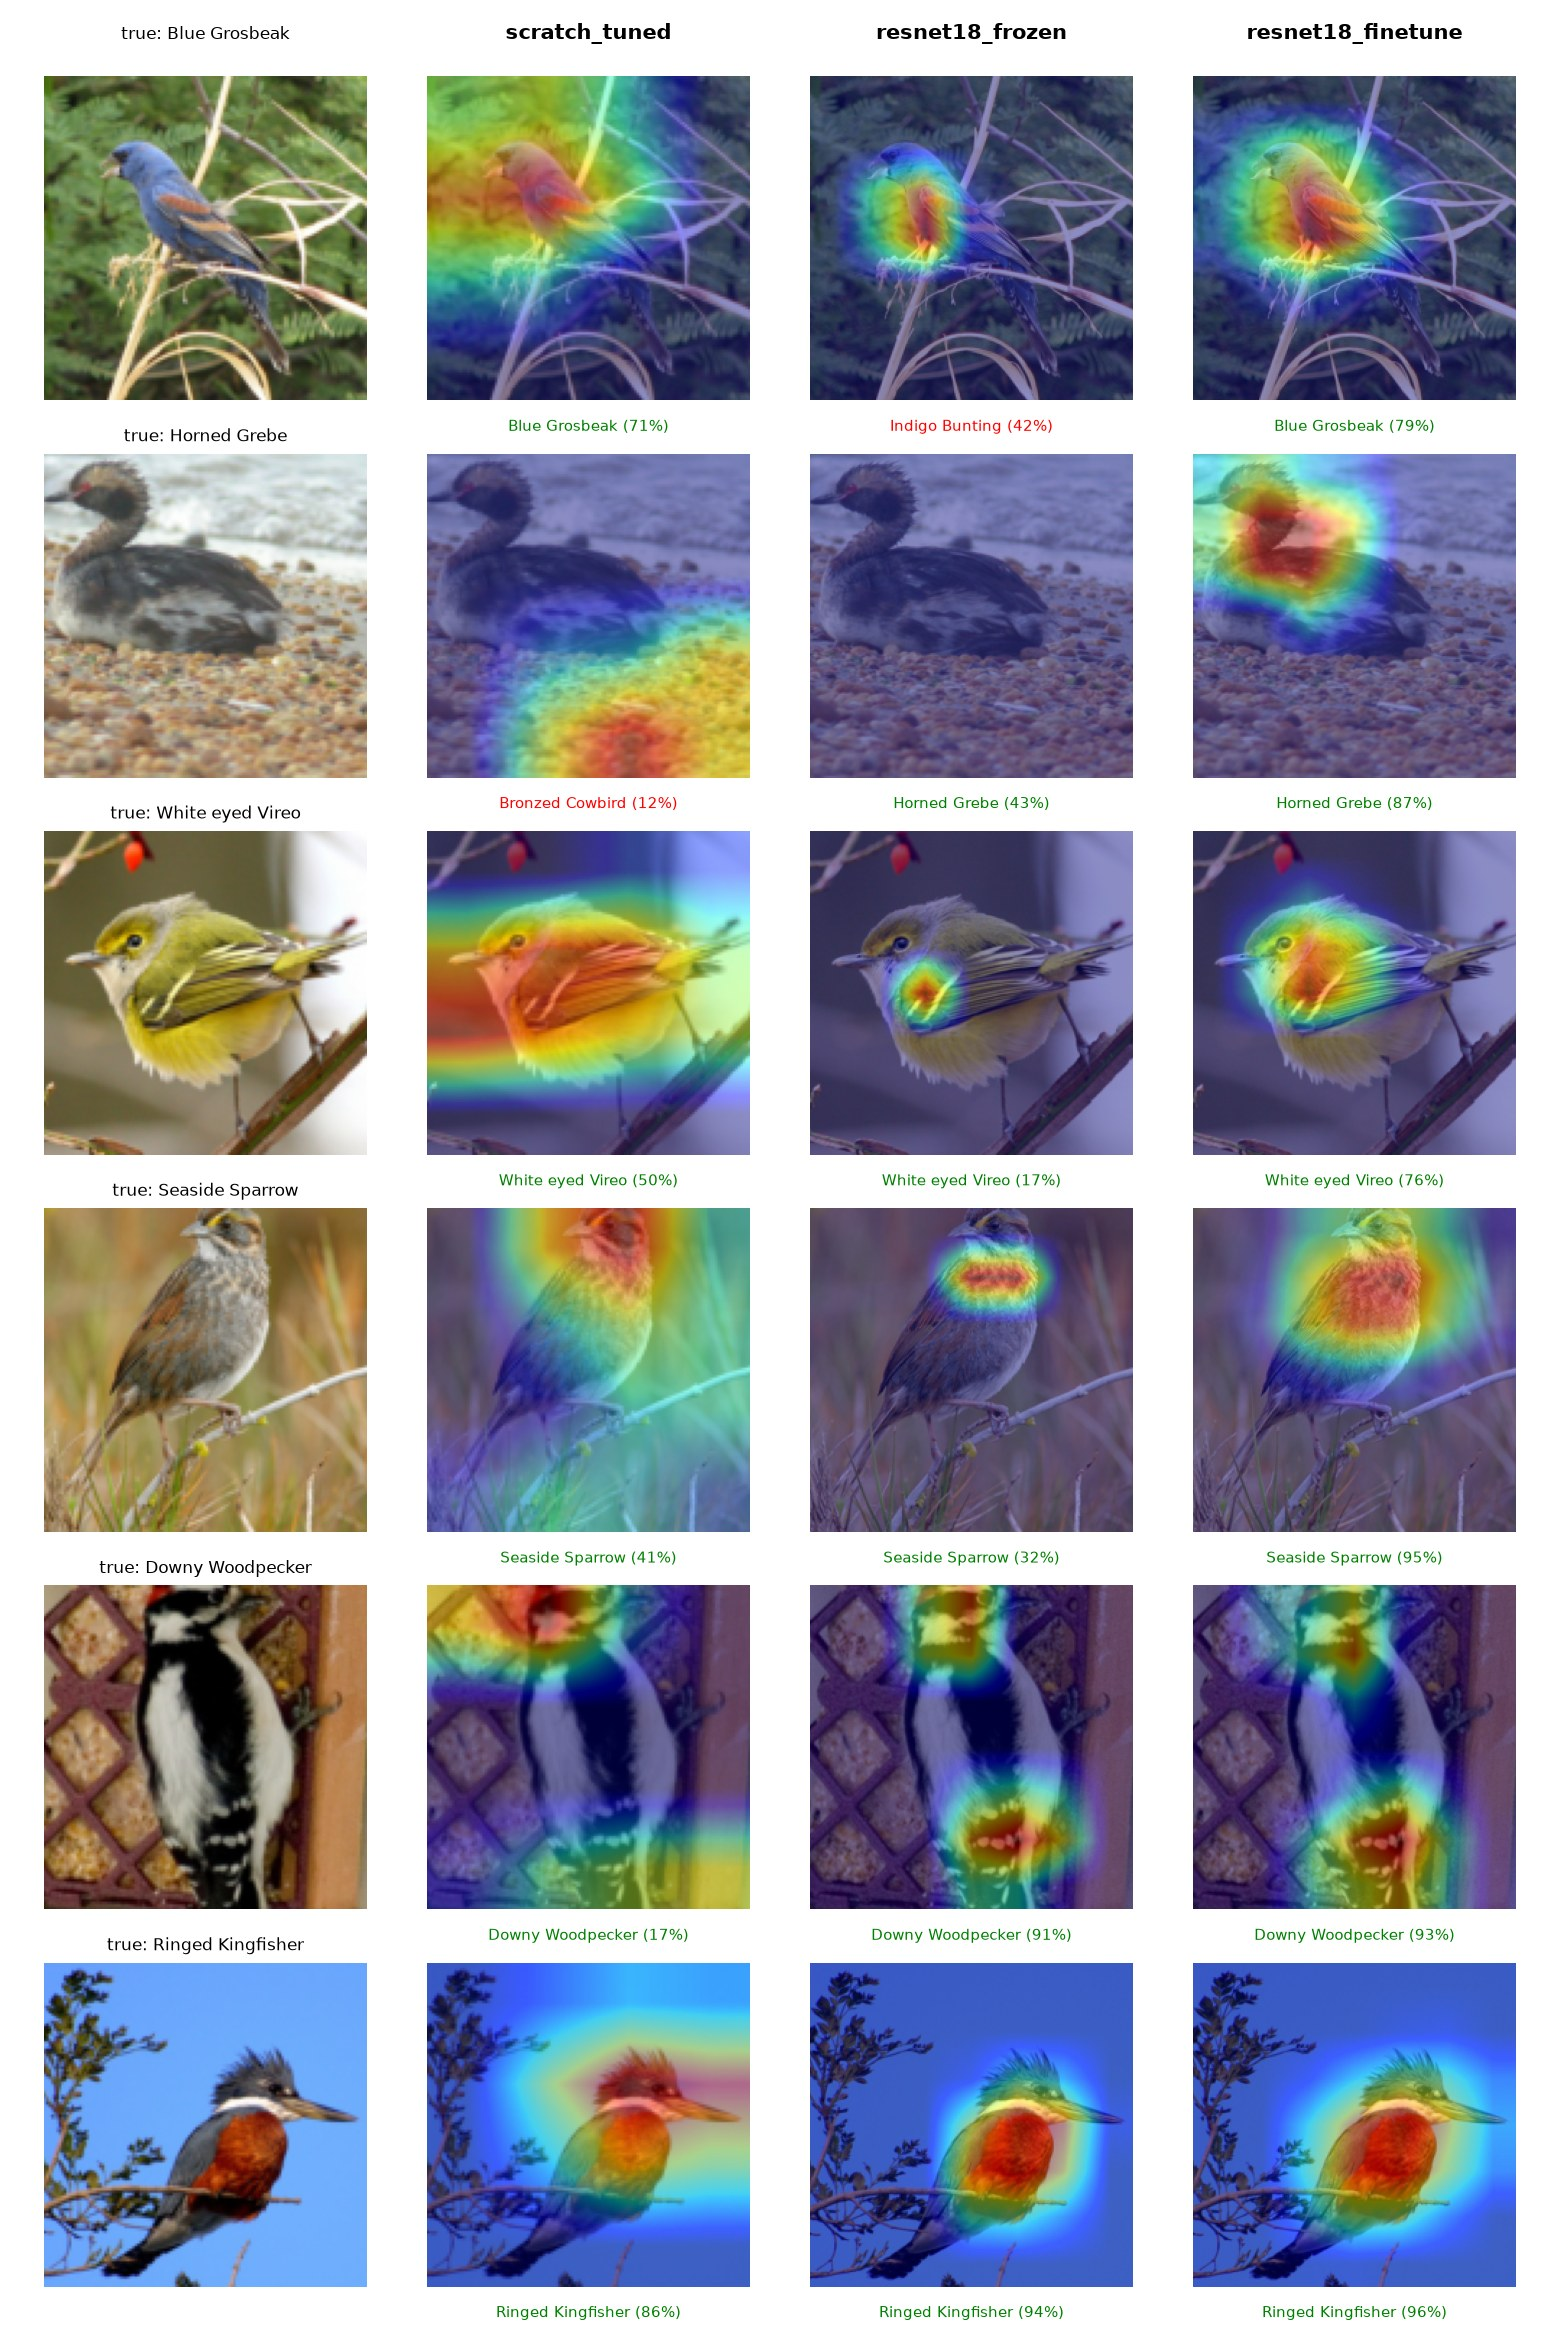
\includegraphics[width=0.85\linewidth]{gradcam_comparison.jpg}
\caption{The same validation images explained by the three final models. Green
labels are correct predictions, red labels wrong ones.}
\label{fig:gradcam_compare}
\end{figure}

\paragraph{Comparison of the models (Figure~\ref{fig:gradcam_compare}).}
\begin{itemize}
  \item The \textbf{fine-tuned ResNet-18} attends to the bird in every row,
        usually its head and breast, with high confidence (76--96\%).
  \item The \textbf{frozen ResNet-18} focuses on small, specific regions (the
        Seaside Sparrow's throat, the Vireo's chest). Its error is telling: it
        calls a Blue Grosbeak an Indigo Bunting, a very similar blue bird,
        because generic ImageNet features find the right region but cannot
        separate close species. For the Horned Grebe its heatmap is empty: no
        region supports the predicted class strongly, a known limitation of
        Grad-CAM.
  \item The \textbf{scratch CNN} gets five of the six images right and often
        looks at the bird (the Kingfisher's crest, the Sparrow's head), but its
        heatmaps are broad and spill into the background. For the Horned Grebe
        it looks at the \emph{pebbles} under the bird and is wrong. The untuned
        baseline relied on background even more: it predicted waterbirds from
        the water around them.
\end{itemize}

\begin{figure}[H]
\centering
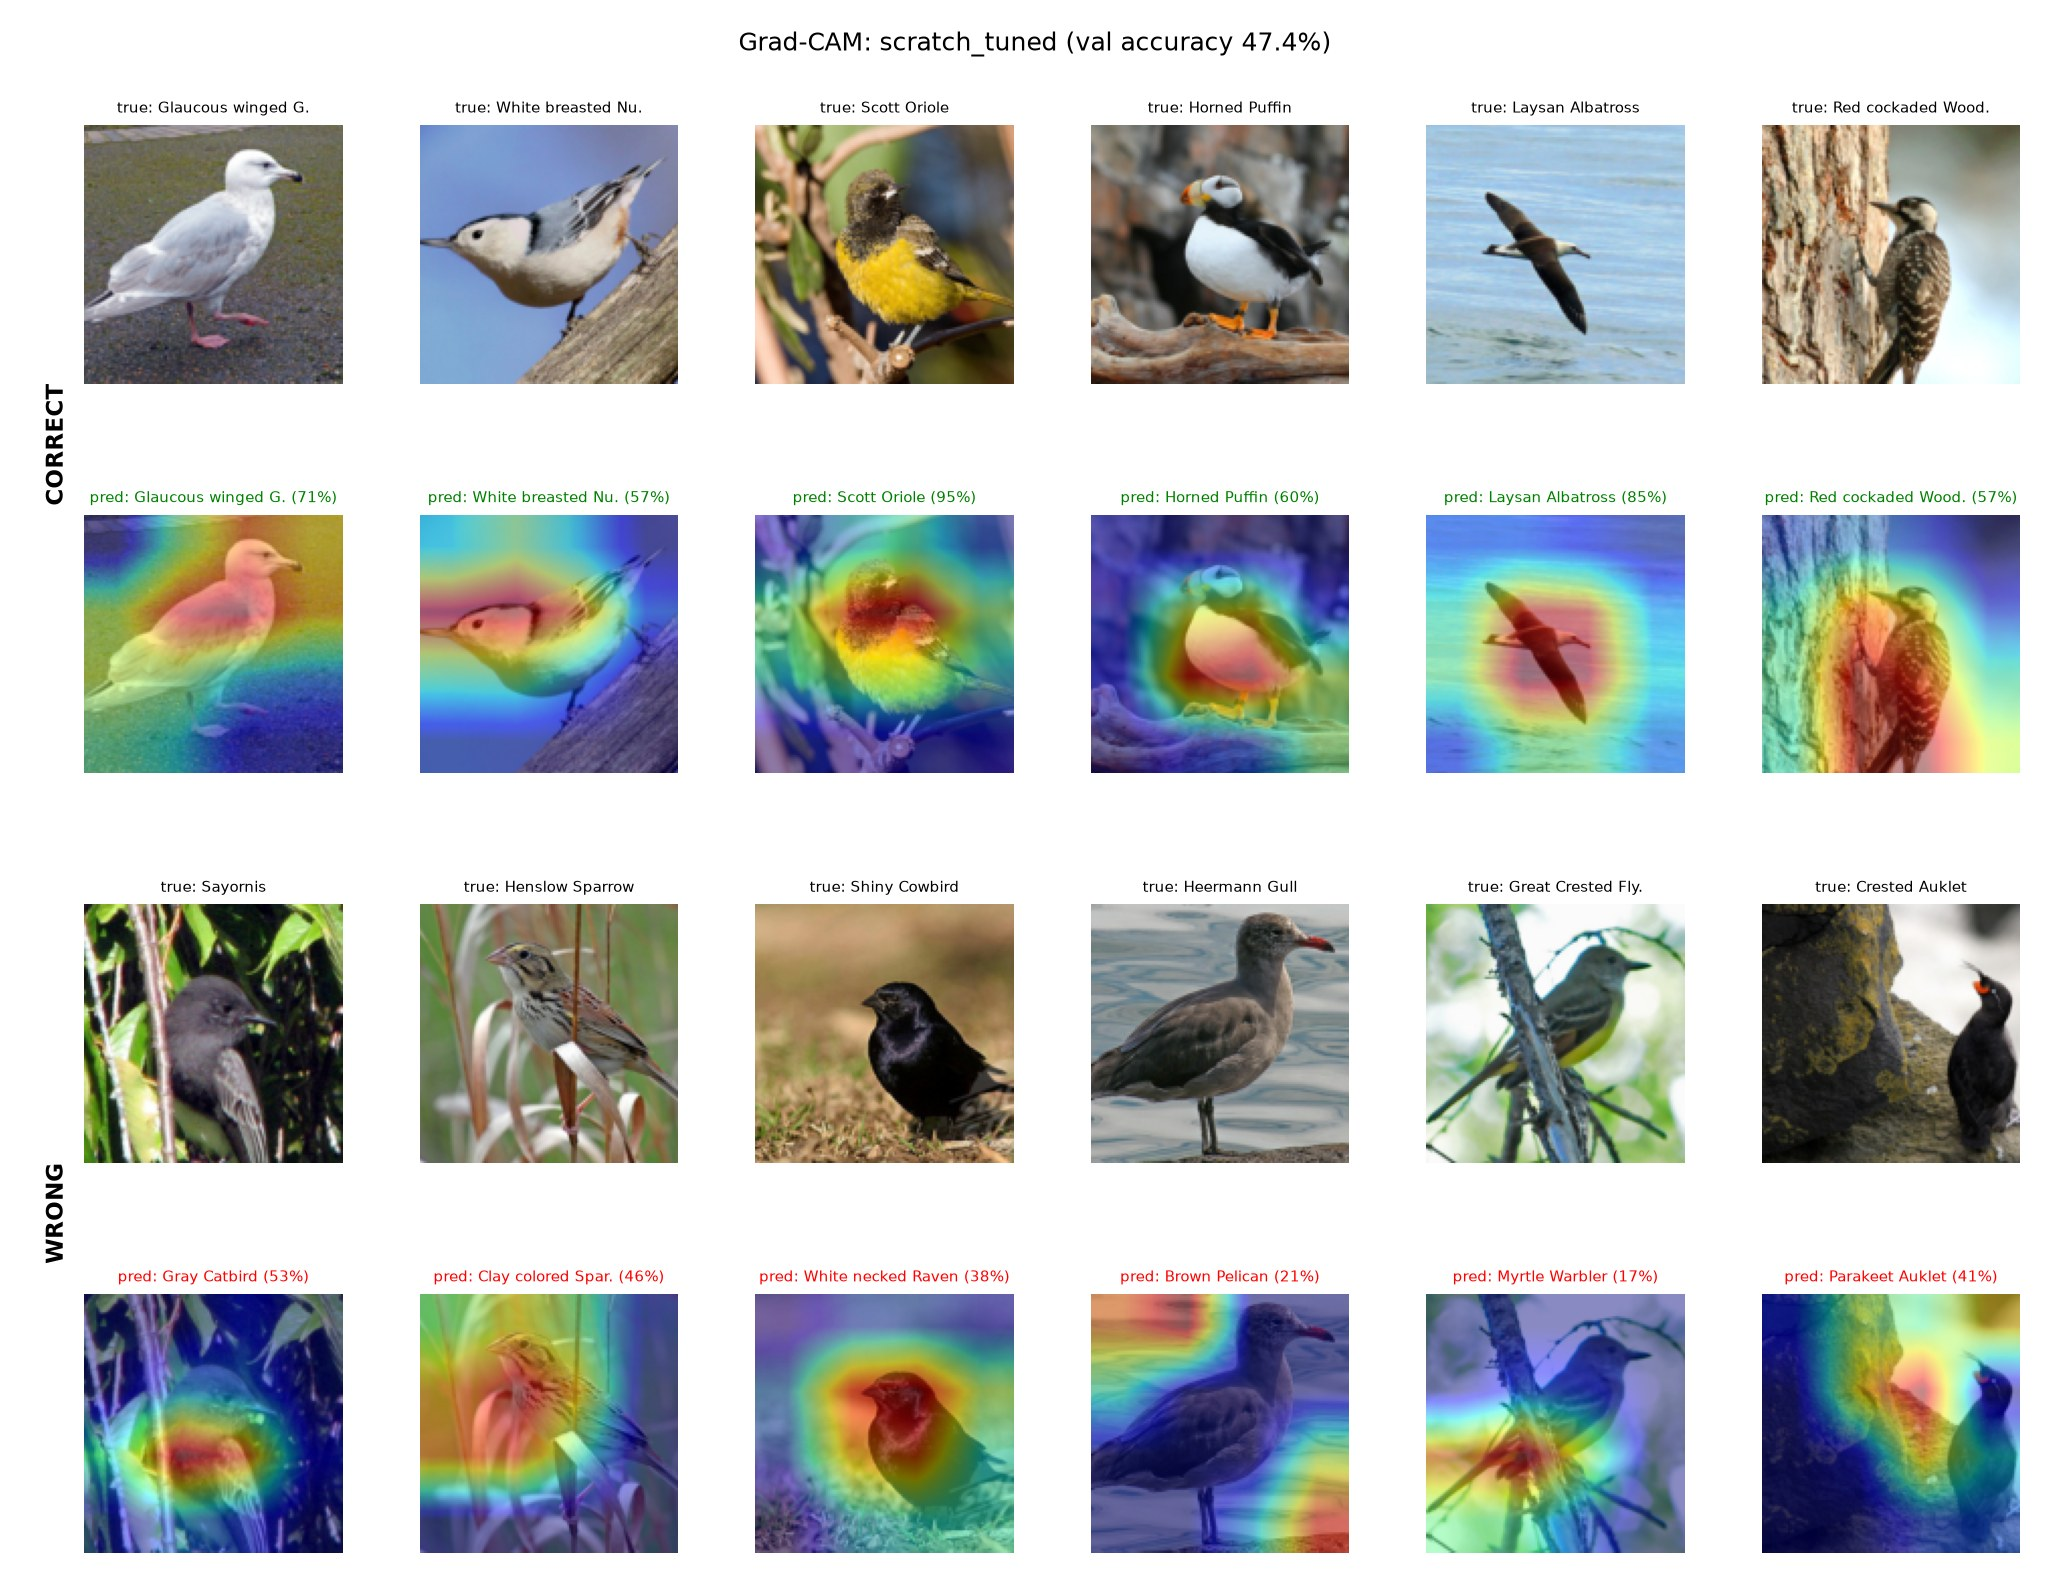
\includegraphics[width=0.9\linewidth]{gradcam_scratch_tuned.jpg}
\caption{Scratch CNN (tuned): six correct and six wrong validation predictions.}
\label{fig:gradcam_scratch}
\end{figure}

\paragraph{Scratch CNN, correct vs.\ wrong (Figure~\ref{fig:gradcam_scratch}).}
Correct predictions mostly centre on the bird (the Scott Oriole at 95\%, the
Laysan Albatross at 85\%). Wrong predictions fall into two groups.
\emph{Background shortcuts:} the Heermann Gull is called a Brown Pelican while
the heatmap sits on the water, the Great Crested Flycatcher becomes a Myrtle
Warbler with the heatmap on the branch, and the Crested Auklet is judged from
the rock beside it. \emph{Similar species:} Henslow Sparrow vs.\ Clay-colored
Sparrow, and a Shiny Cowbird called a White-necked Raven (both all-black). The
wrong predictions also have low confidence (17--53\%).

\begin{figure}[H]
\centering
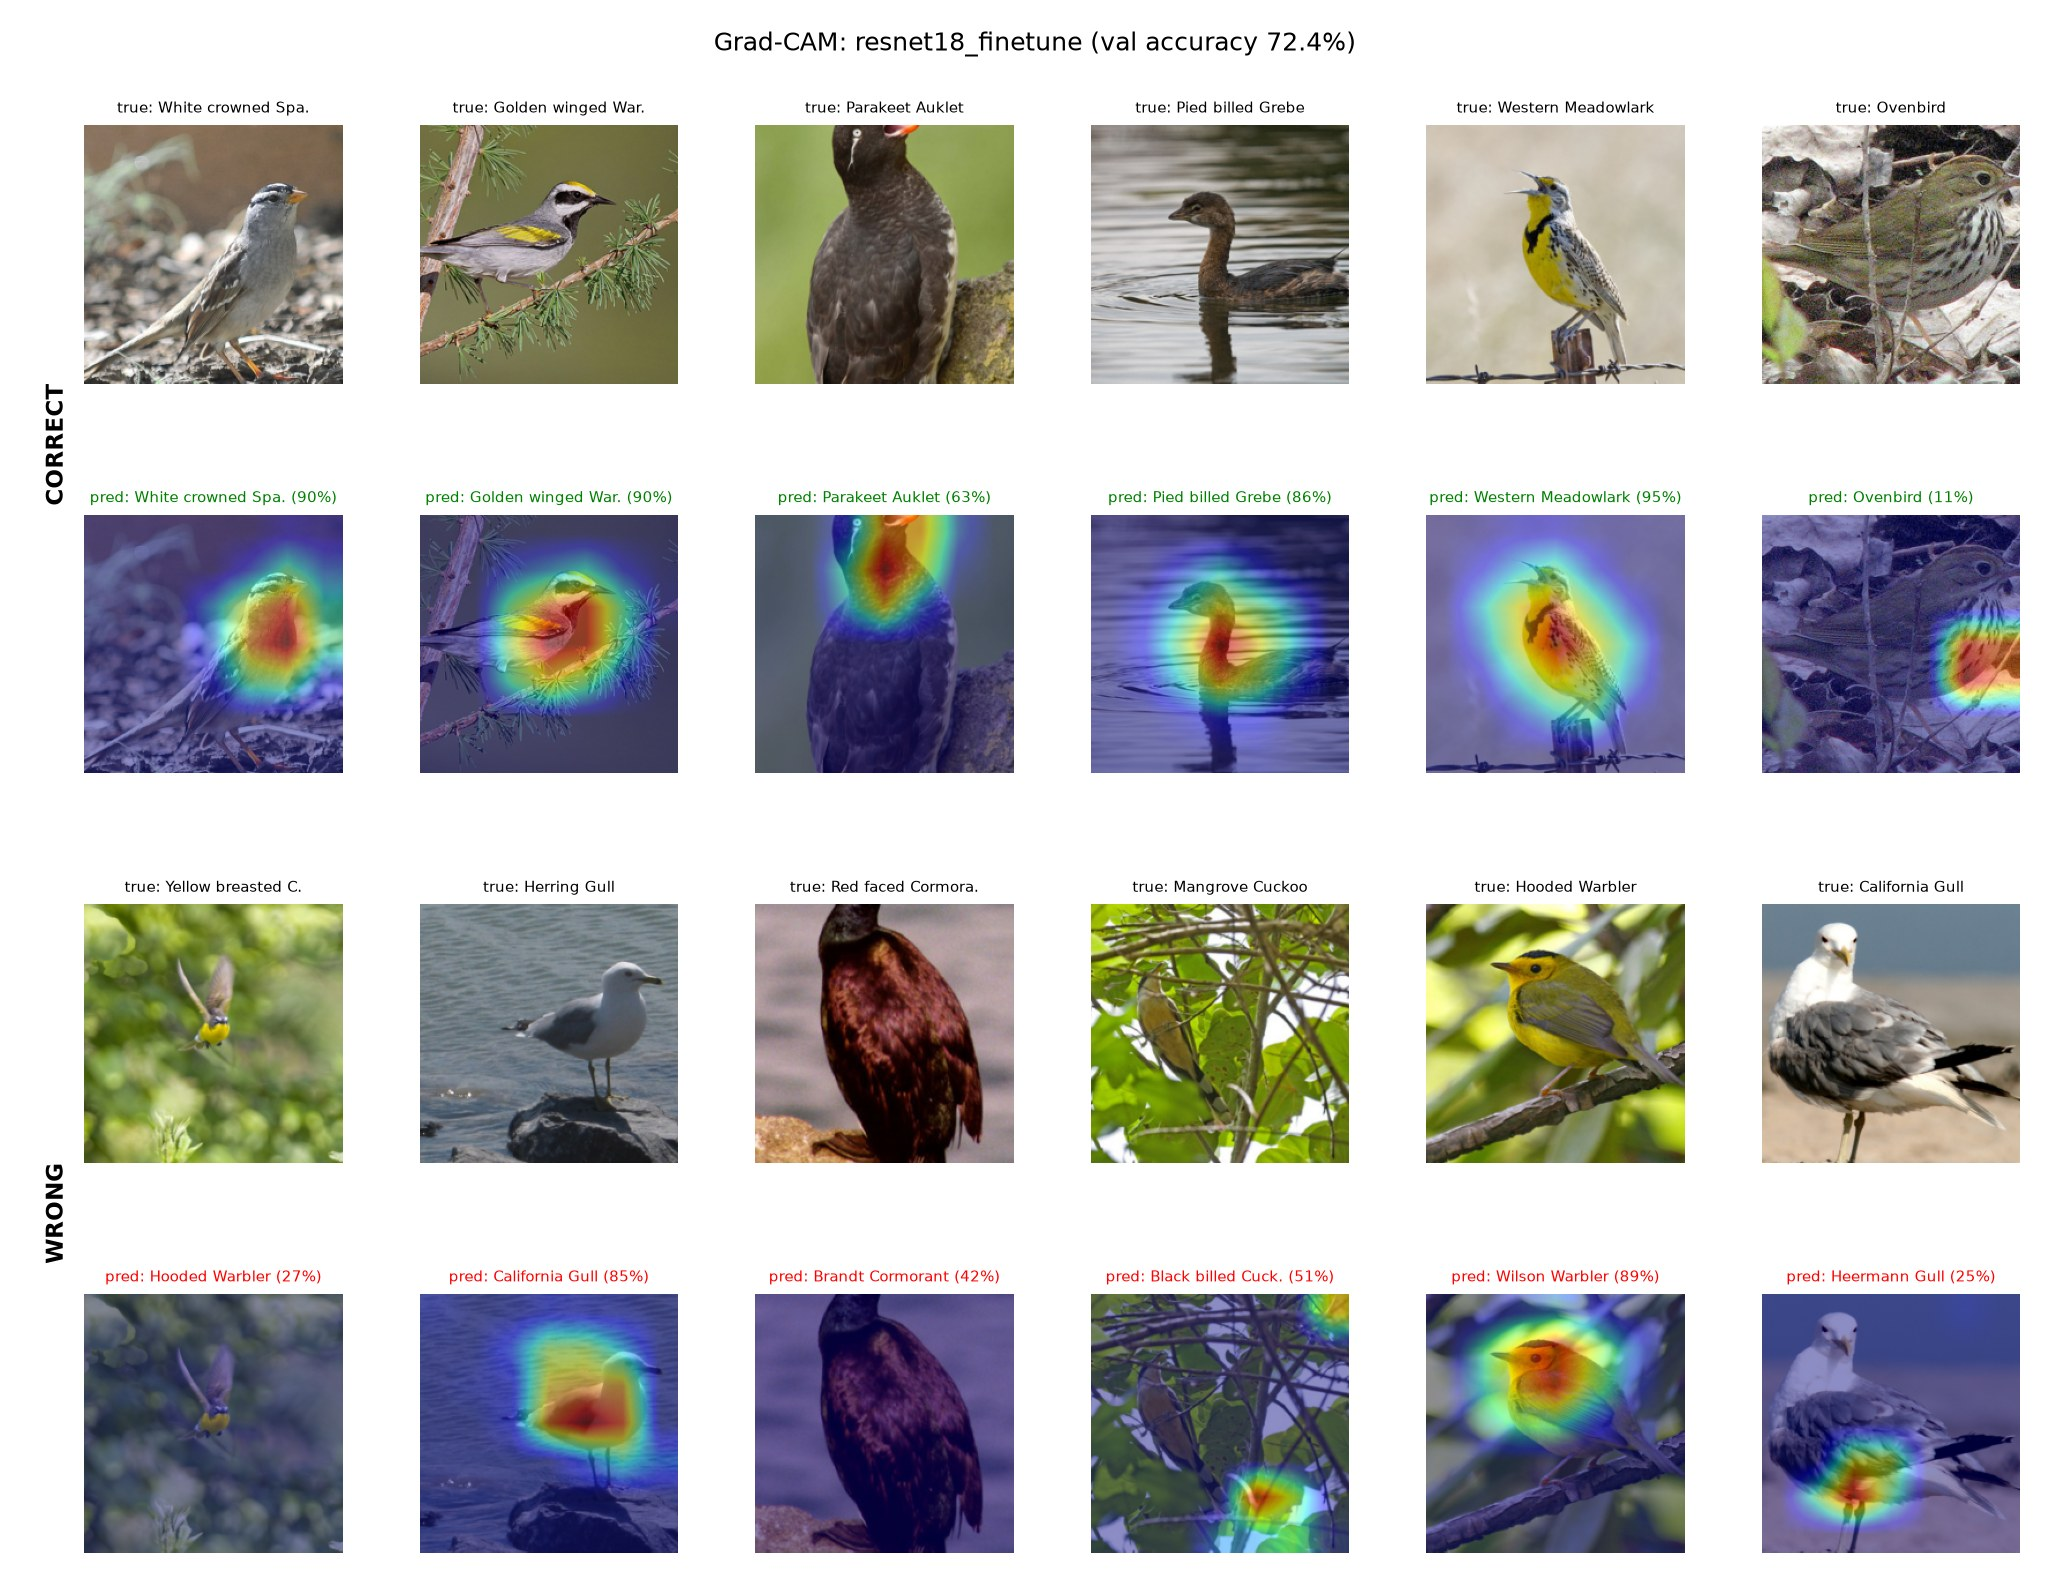
\includegraphics[width=0.9\linewidth]{gradcam_resnet18_finetune.jpg}
\caption{ResNet-18 fine-tuned: six correct and six wrong validation predictions.}
\label{fig:gradcam_resnet}
\end{figure}

\paragraph{Fine-tuned ResNet-18, correct vs.\ wrong (Figure~\ref{fig:gradcam_resnet}).}
Correct predictions focus tightly on the head and breast, where the
species-defining marks are (the White-crowned Sparrow's head stripes, the
Meadowlark's black V). Most errors are between \emph{near-identical species}
while the model still looks at the bird: Herring Gull vs.\ California Gull,
Hooded Warbler vs.\ Wilson's Warbler (with 89\% confidence), Red-faced vs.\
Brandt's Cormorant. The remaining errors come from \emph{hard images}: a
small flying Yellow-breasted Chat with almost no heatmap, and a Mangrove Cuckoo
mostly hidden by leaves, where the model looks at the branches. One correct
prediction (Ovenbird, 11\%) is right with very low confidence while looking at
the edge of the bird rather than its distinctive head and breast, so not every
correct answer is correct for a convincing reason.

%=====================================================================
\section{Benchmarking}
%=====================================================================

\paragraph{Published results.} Our test numbers use the official CUB test split
(minus the one leaked image) and top-1 accuracy, the standard metric for this
dataset, so they are comparable in split and metric. Reported results include
\todo{verify each number against the original paper before submission}:
\begin{itemize}
  \item a fine-tuned ResNet-50 at 448-pixel input: about 84.5\%;
  \item Bilinear CNN~\cite{lin2015}: 84.1\%;
  \item TransFG, a Vision Transformer method~\cite{he2022transfg}: 91.7\%.
\end{itemize}
Our fine-tuned ResNet-18 (74.4\%) is about 10 points below the ResNet-50
baseline. The difference has clear causes: a smaller backbone (11\,M vs.\
24\,M parameters), half the input resolution (224 vs.\ 448 pixels, which
matters for small details such as eye rings and wing bars), only 15 epochs, and
no fine-grained techniques. Methods in the 90\% range add attention to
discriminative parts and transformer backbones pretrained on much larger data.

\paragraph{Another team.} We also compared against another team's validation
results on the same dataset (their own random 80/20 split, about 1,200
validation images):

\begin{table}[H]
\centering
\caption{Validation accuracy compared with another team (different splits;
indicative only).}
\label{tab:otherteam}
\resizebox{\linewidth}{!}{%
\begin{tabular}{lcc}
\toprule
Setting & Other team & Ours \\
\midrule
Scratch CNN & 9.4\% (0.44\,M params, 20 epochs) & \textbf{47.4\%} (4.82\,M params, tuned, 60 epochs) \\
Frozen encoder & 58.3\% (ResNet-50) & \textbf{60.7\%} (ResNet-18) \\
Partially fine-tuned & 72.3\% (ResNet-50) & --- \\
Fully fine-tuned & \textbf{74.3\%} (ResNet-50) & 72.4\% (ResNet-18) \\
Top-5, fully fine-tuned & 92.5\% & 92.1\% \\
\bottomrule
\end{tabular}}
\end{table}

The comparison is not fully fair --- different validation images, unknown
input sizes and no test results on their side --- so differences of one or two
points are within noise. Two conclusions still hold. First, their scratch CNN
underfits (10.9\% training accuracy), while ours reaches 96\%; model capacity,
batch normalization and the learning-rate tuning make the difference. Second,
ResNet-50 is only about 2 points better than our ResNet-18 at twice the size,
suggesting that at 224 pixels resolution and pretraining matter more than
depth.

%=====================================================================
\section{Final Model Selection}
%=====================================================================

\textbf{Classification encoder: ResNet-18, fine-tuned.} It has the best score on
every metric (74.4\% test accuracy, 0.743 macro F1, 92.3\% top-5), it is the
only model whose Grad-CAM consistently looks at the bird, and it trains in
about 4 minutes. Its 512-channel 7$\times$7 feature map is the encoder we plan
to reuse in Milestone~2. The tuned scratch CNN (49.6\%) remains the
from-scratch baseline.

Colorization and captioning models will be selected in Milestone~2.

%=====================================================================
\section{Failures and Limitations}
%=====================================================================

\begin{itemize}
  \item \textbf{Overfitting of the scratch CNN.} 96\% training vs.\ 47\%
        validation accuracy. With $\sim$24 images per species, the model
        memorises. Next we would try stronger augmentation (larger crop range,
        random erasing), more dropout, or mixup.
  \item \textbf{Background shortcuts.} Grad-CAM shows the scratch model still
        uses water, rocks and branches as cues. Object-centred cropping (the
        original CUB bounding boxes) could reduce this.
  \item \textbf{The default learning rate was too high.} Our first scratch run
        used 0.001 and reached 31.9\%; tuning found 0.0003 (+7 points). The
        best value was also at the edge of the first search range, which we
        only discovered and fixed with the coarse-to-fine search.
  \item \textbf{Random search underperformed} for this two-parameter problem
        because its draws missed the low learning-rate region.
  \item \textbf{Small validation set.} $\pm$1.4 points of noise makes small
        differences (e.g.\ between weight-decay values) inconclusive.
  \item \textbf{Low resolution.} 128 pixels for the scratch model and 224 for
        ResNet-18 lose fine details; published results use 448.
  \item \textbf{Single seed.} Every result comes from one run (seed 42); we did
        not measure run-to-run variance.
  \item Next steps for the encoder: higher resolution, a larger or
        transformer backbone, and partial fine-tuning as a middle ground
        between frozen and full fine-tuning.
\end{itemize}

%=====================================================================
\section{Team Contributions}
%=====================================================================

\todo{describe who did what, consistent with each member's GitHub commits}

\begin{itemize}
  \item \textbf{Mohamed Wael ElHadary} --- \todo{contributions}
  \item \textbf{Kerolos Bassem} --- \todo{contributions}
  \item \textbf{Andrea} --- \todo{contributions}
\end{itemize}

%=====================================================================
\begin{thebibliography}{99}
%=====================================================================

\bibitem{wah2011}
C.~Wah, S.~Branson, P.~Welinder, P.~Perona and S.~Belongie.
\newblock The Caltech-UCSD Birds-200-2011 Dataset.
\newblock Technical Report CNS-TR-2011-001, California Institute of Technology, 2011.

\bibitem{reed2016}
S.~Reed, Z.~Akata, H.~Lee and B.~Schiele.
\newblock Learning Deep Representations of Fine-Grained Visual Descriptions.
\newblock In \emph{CVPR}, 2016.

\bibitem{he2016}
K.~He, X.~Zhang, S.~Ren and J.~Sun.
\newblock Deep Residual Learning for Image Recognition.
\newblock In \emph{CVPR}, 2016.

\bibitem{deng2009}
J.~Deng, W.~Dong, R.~Socher, L.-J.~Li, K.~Li and L.~Fei-Fei.
\newblock ImageNet: A Large-Scale Hierarchical Image Database.
\newblock In \emph{CVPR}, 2009.

\bibitem{ioffe2015}
S.~Ioffe and C.~Szegedy.
\newblock Batch Normalization: Accelerating Deep Network Training by Reducing
Internal Covariate Shift.
\newblock In \emph{ICML}, 2015.

\bibitem{loshchilov2019}
I.~Loshchilov and F.~Hutter.
\newblock Decoupled Weight Decay Regularization.
\newblock In \emph{ICLR}, 2019.

\bibitem{loshchilov2017}
I.~Loshchilov and F.~Hutter.
\newblock SGDR: Stochastic Gradient Descent with Warm Restarts.
\newblock In \emph{ICLR}, 2017.

\bibitem{szegedy2016}
C.~Szegedy, V.~Vanhoucke, S.~Ioffe, J.~Shlens and Z.~Wojna.
\newblock Rethinking the Inception Architecture for Computer Vision.
\newblock In \emph{CVPR}, 2016.

\bibitem{bergstra2012}
J.~Bergstra and Y.~Bengio.
\newblock Random Search for Hyper-Parameter Optimization.
\newblock \emph{Journal of Machine Learning Research}, 13:281--305, 2012.

\bibitem{selvaraju2017}
R.~R.~Selvaraju, M.~Cogswell, A.~Das, R.~Vedantam, D.~Parikh and D.~Batra.
\newblock Grad-CAM: Visual Explanations from Deep Networks via Gradient-based
Localization.
\newblock In \emph{ICCV}, 2017.

\bibitem{lin2015}
T.-Y.~Lin, A.~RoyChowdhury and S.~Maji.
\newblock Bilinear CNN Models for Fine-grained Visual Recognition.
\newblock In \emph{ICCV}, 2015.

\bibitem{he2022transfg}
J.~He, J.-N.~Chen, S.~Liu, A.~Kortylewski, C.~Yang, Y.~Bai and C.~Wang.
\newblock TransFG: A Transformer Architecture for Fine-Grained Recognition.
\newblock In \emph{AAAI}, 2022.

\bibitem{mlflow}
MLflow: An open source platform for the machine learning lifecycle.
\newblock \url{https://mlflow.org}.

\bibitem{pytorch}
A.~Paszke et al.
\newblock PyTorch: An Imperative Style, High-Performance Deep Learning Library.
\newblock In \emph{NeurIPS}, 2019.

\end{thebibliography}

\end{document}
